\documentclass[]{report}
\usepackage[hmargin=1.25in,vmargin=1in]{geometry} %调整页边距
% \usepackage[inner=1in,outer=1.25in]{geometry} %书籍左右不等宽排版
\usepackage[utf8]{inputenc}
% \usepackage[]{ctex} %据说可以直接调用诸如 \kaishu \fangsong \heiti 的命令修改字体
\usepackage[]{xeCJK}
\setCJKmainfont[BoldFont = STHeiti, ItalicFont = STKaiti]{Songti SC Light} %中文主字体
\setCJKsansfont[BoldFont = Weibei SC, ItalicFont = Xingkai SC Light]{Xingkai SC} %中文无衬线字体
\setCJKmonofont[BoldFont = Libian SC, ItalicFont = STFangsong]{Yuanti SC Light} %中文等宽字体
\setmainfont{Times New Roman} %\rmfamily
\setsansfont{Comic Sans MS} %\sffamily
\setmonofont{Courier} %\ttfamily

\usepackage{ulem} %解决下划线、删除线之类的
\usepackage{bookmark}

\usepackage{lipsum} %填充文本

\usepackage{amsmath} %数学公式问题
\usepackage{amsthm} %公式环境,如proof
\usepackage{booktabs} %三线表
\usepackage{mathrsfs} %在公式里面使用那个最花的字体
\usepackage{amssymb} %公式里面用空心黑体和旧式字体
\usepackage{amssymb} %AMS符号
\usepackage{amsthm} %AMS定理环境

\usepackage{markdown} %使用markdown语法,在编译时需要打开 shell-escape 标记,即 $ xelatex --shell-escape example.tex
\markdownSetup{hashEnumerators = true} %允许使用 #. 的方式编写有序列表
\markdownSetup{inlineFootnotes = true} %允许使用脚注形式的超链接,调用语法为 [anchor](uri), ^[footnote], <uri>
\markdownSetup{fencedCode = true} %以反引号和缩进来插入代码段,相当于 verbatim
\markdownSetup{
  pipeTables = true
} %支持表格的用法 (图片已经在markdown包里面支持了)
% \usepackage{booktabs} %解决三线表的线条粗细问题

\usepackage{graphicx} %插入图片
\usepackage{pdfpages} %插入PDF文件
\usepackage{makeidx}

\usepackage{tikz} %带圈字符
\usepackage{etoolbox} %带圈字符 (提供robustify)
\usepackage{enumitem}
\newcommand*{\circled}[1]{\lower.7ex\hbox{\tikz\draw (0pt, 0pt)%
    circle (.5em) node {\makebox[1em][c]{\small #1}};}} %新定义命令:带圈字符
\robustify{\circled}
% \usepackage{enumerate} %有序列表

\usepackage{hyperref} %超链接
% \usepackage[hidelinks]{hyperref} %隐藏超链接的红框
\markdownSetup{
  inlineFootnotes = true,
  renderers = {
    link = {\href{#3}{#1}},
  }
} % markdown块中使用直接点进去的超链接
% \setlist[enumerate,1]{label=(\arabic*).,font=\textup,leftmargin=7mm,labelsep=1.5mm,topsep=0mm,itemsep=-0.8mm}
% \setlist[enumerate,2]{label=(\alph*).,font=\textup,leftmargin=7mm,labelsep=1.5mm,topsep=-0.8mm,itemsep=-0.8mm}

\title{组成原理笔记}
\author{上官凝}
\date{\today}

\linespread{1.3} %行间距为1.3倍默认间距 (1.3 x 1.2倍字符宽度)

\makeindex

\begin{document}
	\theoremstyle{definition} \newtheorem{theorem}{Thm}[section] %定义一个定理Thm,序号为section的下一级序号
	\theoremstyle{definition} \newtheorem{definition}{Def}[section] %定义一个定义Def,序号为section的下一级序号
	\theoremstyle{plain} \newtheorem{lemma}{lemma}[section] %引理

	\maketitle
	\newpage

	\tableofcontents
	\newpage

	\section{序幕}
	组成原理的实验很重要。它会让你对这门课学的有一个比较深入的理解。在写CPU的时候多翻COD书,可以参考我在GitHub上的代码(Username:OrigamiAyc)。所有的策略都会有不同场景下的tradeoff,最好思考一下优缺点和适用范围。图片的位置可能会有偏移(当这一页放不下就会挪到下一页正文当中,但是与正文的相对位置就改变了),请以图片标题为准

	\section{计算需要用的公式}
	\begin{enumerate}[label = \textsf{\arabic{*}}]
		\item 运算速度与处理器性能:(这里需要注意机器周期和时钟周期\textbf{未必相等})\par
		\begin{enumerate}
			\item CPI:指令周期,表示执行一条指令所需的平均时钟周期数,即\[\frac{\mbox{执行程序所需CPU时钟周期数}}{\mbox{程序包含的指令条数}}\]
			\item MIPS:百万条指令每秒,即单位时间内执行的指令数,即\[\frac{\mbox{程序的指令条数}}{\mbox{程序的执行时间}\times10^6}\]
			\item MFLOPS:百万次浮点操作每秒,用来衡量机器浮点运算的性能,即\[\frac{\mbox{程序的浮点操作次数}}{\mbox{程序的执行时间}\times10^6}\]注意这里计算的指包括浮点运算次数,却除以的是总时间
			\item 时间计算公式(IC是程序执行过程中所处理的指令数):\[\begin{aligned} \mathrm{T_{CPU}}=\ &\mathrm{CPI}\times\mathrm{IC}\times\mathrm{T_{CLK}}\\ =\ &\sum(\mathrm{CPI_i}\times\mathrm{IC_i})\times\mathrm{T_{CLK}}\end{aligned}\]
			\item Gibson法求平均CPI:\[\overline{\mathrm{CPI}}=\sum(\mathrm{IC_i/IC})\times \mathrm{CPI_i}\]注意在指令集改变之后,有可能会出现所有指令所占比例加起来不等于100\%的情况,例如ch1 page 68-70例1\footnote{这个例子的答案有坑,$\times$恰好标在了正确答案的位置,建议听课}
			\item 性能与响应时间(从事件开始到结束之间的时间)成反比,与吞吐率(在单位时间内所能完成的工作量(任务) (多用户系统))	不同
			\item 可靠性与可用率:可靠性用平均无故障运行时间(MTBF)衡量,可用率为 MTBF/(MTBF + MTTR)(平均故障修复时间)
		\end{enumerate}
		\item Amdahl定律:适用于改进一段系统的一部分,用于计算改进之后的执行总时间。\[\begin{gathered}
			T_e=T_0[(1-f_e)+\frac{f_e}{S_e}]\\
			S=\frac{1}{(1-f_e)+\frac{f_e}{S_e}}\\
			f_e=T_1/T_0\qquad S_e=T_1/T_2
		\end{gathered}\]其中$T_0,T_1,T_2,T_e$分别原总时长、原改进段时长、新改进段时长、新总时长,$f_e,S_e$分别为可改进比例与部件加速比,S为总加速比。理解阿姆达尔定律的计算实质,即\textit{加速比 = 增强前时间/增强后时间},可以计算同时多个优化
		\item 计算总共可能有多少种X地址指令:指令字长$n$,可选有$2^n$种指令,若不定长指令,比如4个bit的op code是二地址,10个bit的op code是一地址,那么用4个bit全是1则为一地址的方式来区分
		\item 单周期CPU确定主频:关键路径法;多周期和流水线都是用时最长的那一段
		\item 流水线最大加速比:流水线站数(ch4 page 13)
		\item 流水线的性能指标:
		\begin{enumerate}
			\item 吞吐率:单位时间内流水线所完成的任务数或输出结果的数量。分各段时间相等和不等来讨论(设$m$为流水深度,$n$为任务数)。
			\begin{table}[h]
				\centering
				\begin{tabular}{ccc}
					\toprule
					&各段时间相等&各段时间不等\\
					\midrule
					最大吞吐率 & $TP_{\max}=1/{\Delta t_0}$ & $TP_{\max}=1/\max{\Delta t_i}$\\
					实际吞吐率 & $TP=\dfrac{TP_{\max}}{1+(m-1)/n}$ & $TP=\dfrac{n}{\sum_{i=1}^m(\Delta t_i)+(n-1)\max\Delta t_i }$\\
					\bottomrule
				\end{tabular}
			\end{table}
			\item 加速比:流水线速度与等功能的非流水线速度之比。若为各段时间相等的情况,加速比 $S=\dfrac{T_{\mbox{非流水}}}{T_{\mbox{流水}}}=\dfrac{m}{1+(m-1)/n}$
			\item 效率:流水线的设备利用率(部件运行时间与总时间的比率,即时空图上阴影部分与大矩形面积之比),$E=\dfrac{1}{1+(m-1)/n}$
			\item 三者关系:效率是实际加速比S与最大加速比m之比;$E=TP\Delta t_0$
		\end{enumerate}
		\item 计算第几个周期在做什么。比如说,在一个\textbf{充分转发并有着异常处理}的流水线CPU里面,给一个汇编段,第四条指令是 \verb|add|,问这个指令算数溢出的时候是第几个周期。算数溢出是EX段,那画一下时空图,就是CC6。在 \verb|add| 之前不巧还有一个 \verb|sw| 于是interlock,再加一个周期,就是CC7。这种题要考虑到各种特殊情况(只存在ALU之间转发、延迟槽以及分支预测、奇怪的结构比如 \verb|beq| 需要三个周期)
		\item 类似的还有判断数据相关。如果有数据通路(可以手画一个draft)可以把寄存器编号标在wire上面,表示在这个时钟周期的时候这上面(应该)跑的是哪一个寄存器的值。简便起见可以把转发之后的结果放上去,就不需要再画一大堆MUX辽
		\item 控制信号的值也可以写上去的诶\dots 以上三点同样适用于人工调试代码,无论是实验还是考试的调试题目,具体写法可以参考下文流水线非精确异常处理的例题(COD 4th page 388)
		\item 评价指标
		\begin{figure}[h]
			\centering
			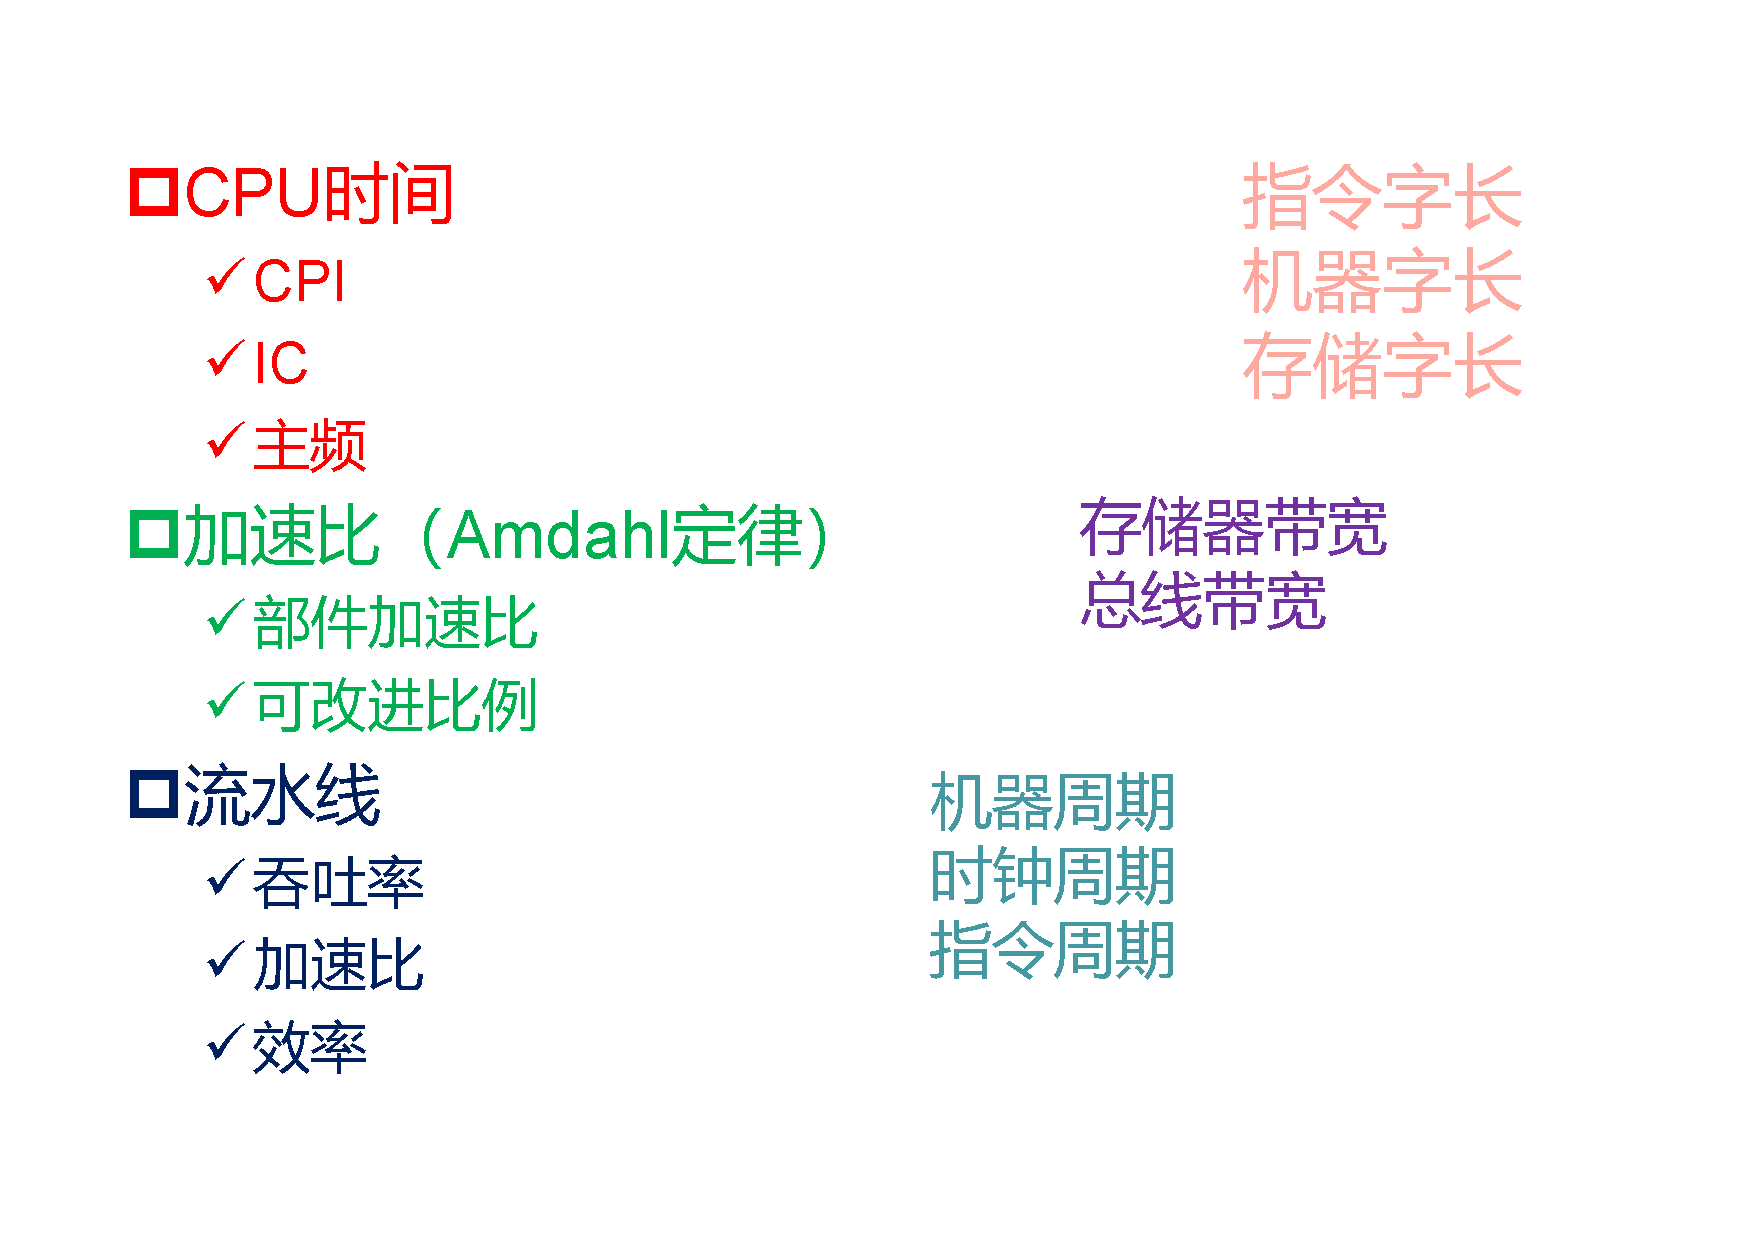
\includegraphics[scale = 0.25]{images/Evaluate.pdf}
			\caption{评价指标}
		\end{figure}
		\item cache性能效率指标:设程序执行过程中,$N_c$表示访问Cache完成存取的总次数,$N_m$表示访问主存完成存取的总次数,则命中率$h=N_c/(N_c+N_m)$;设$t_c$为命中时的Cache访问时间,$t_m$为未命中时的主存访问时间,则Cache/主存平均访问时间$t_a=h\times t_c+(1-h)\times t_m$;用$e$表示访问效率,有$e=\frac{t_c}{t_a}\times100\%$
	\end{enumerate}

	\section{这是一些概念}
	\begin{enumerate}
		\item 机器字长:CPU一次能处理的二进制数据的位数,通常与CPU的寄存器位数有关,多数计算机采用变字长运算
		\item 字:
		\item 机器字长、存储字长、数据字长都是\textbf{字节}的整数倍,不是字
		\item 三二一零地址指令:计算访存次数(取指 + 取操作数/从ACC + 存操作数/存ACC)(4,4/3,2,0)
		\item 指令字长,单位为bit
		\item 地址是无符号整数,但是MIPS指令集里面的I-type指令,其imme/addr段是有符号数,所以能访问的地址量是正负偏移各自$2^15$,加起来$2^16$
		\item 小尾端和大尾端(endians)低/高位字节在低地址
		\begin{figure}[h]
			\centering
			\begin{minipage}{40em}
				\centering
				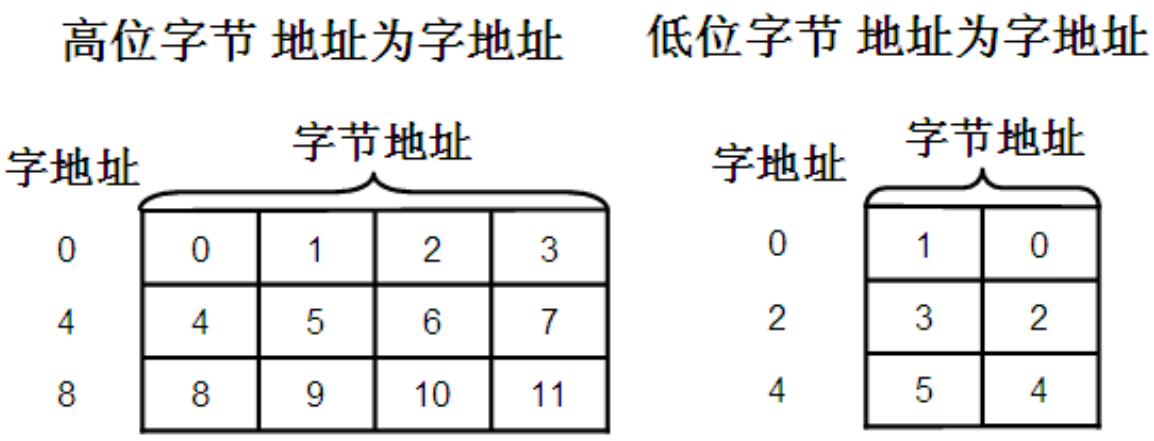
\includegraphics[scale = 0.3]{images/Endians.png}
				\caption{字地址与字节地址}
			\end{minipage}
		\end{figure}
		\item 陷阱:一种意外事故中断,如除0、运算溢出等(ch2.1 page 36)
		\item x86寄存器(见下面的图)
		\begin{figure}[h!]
			\centering
			\begin{minipage}{40em}
				\centering
				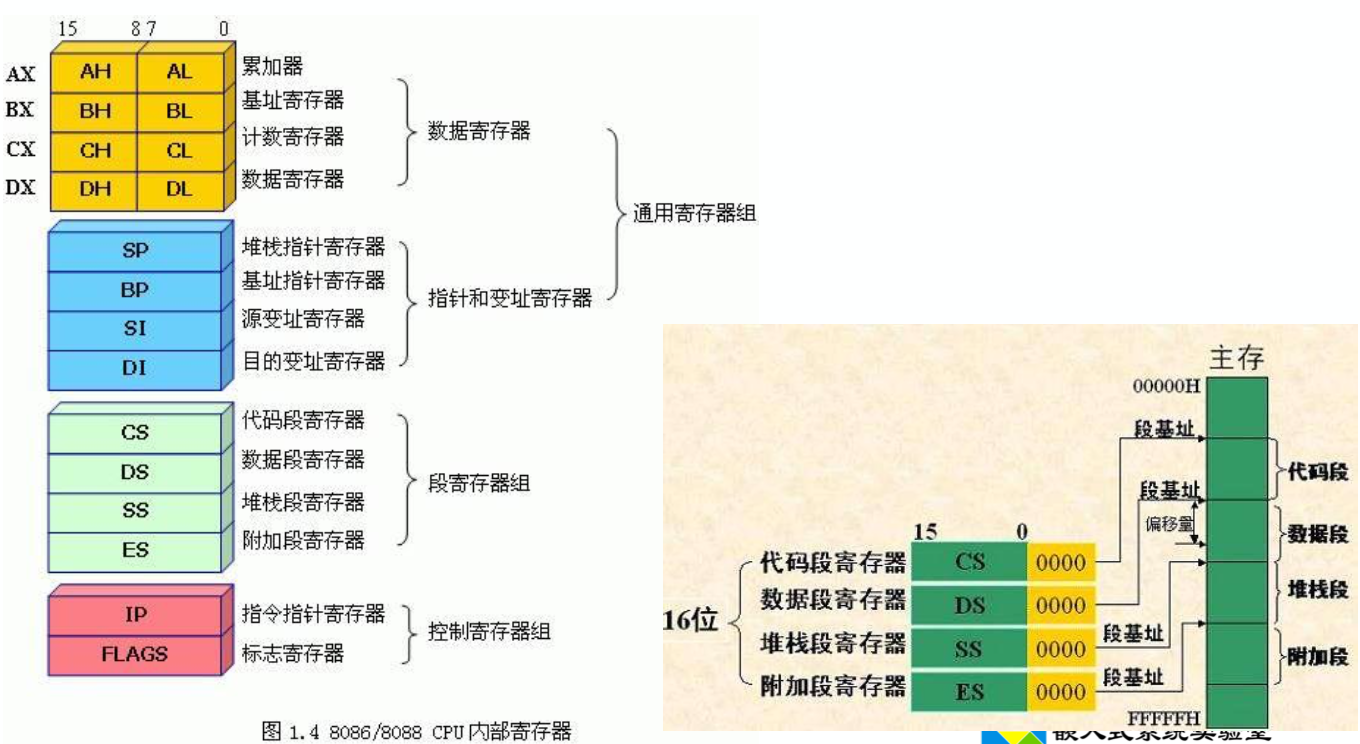
\includegraphics[scale = 0.22]{images/x86.png}
				\caption{x86 registers}
			\end{minipage}
		\end{figure}
		\item 寄存器堆:在一个周期内,某个REG可以同时完成读写操作,但读出的是上一个周期写入的值
		\item 多周期的\verb|beq = PC + offset|,而单周期是\verb|beq = NPC + offset|,这是因为多周期的PC是在从上一条指令的第二个周期保持到自己的第一个周期
		\item MIPS操作数在内存中要字对齐
		\item 程序状态字PSW,记录各种异常的一个数组
		\item 存储器件的Hierarchy以及延迟
		\begin{figure}[h]
			\centering
			\begin{minipage}{40em}
				\centering
				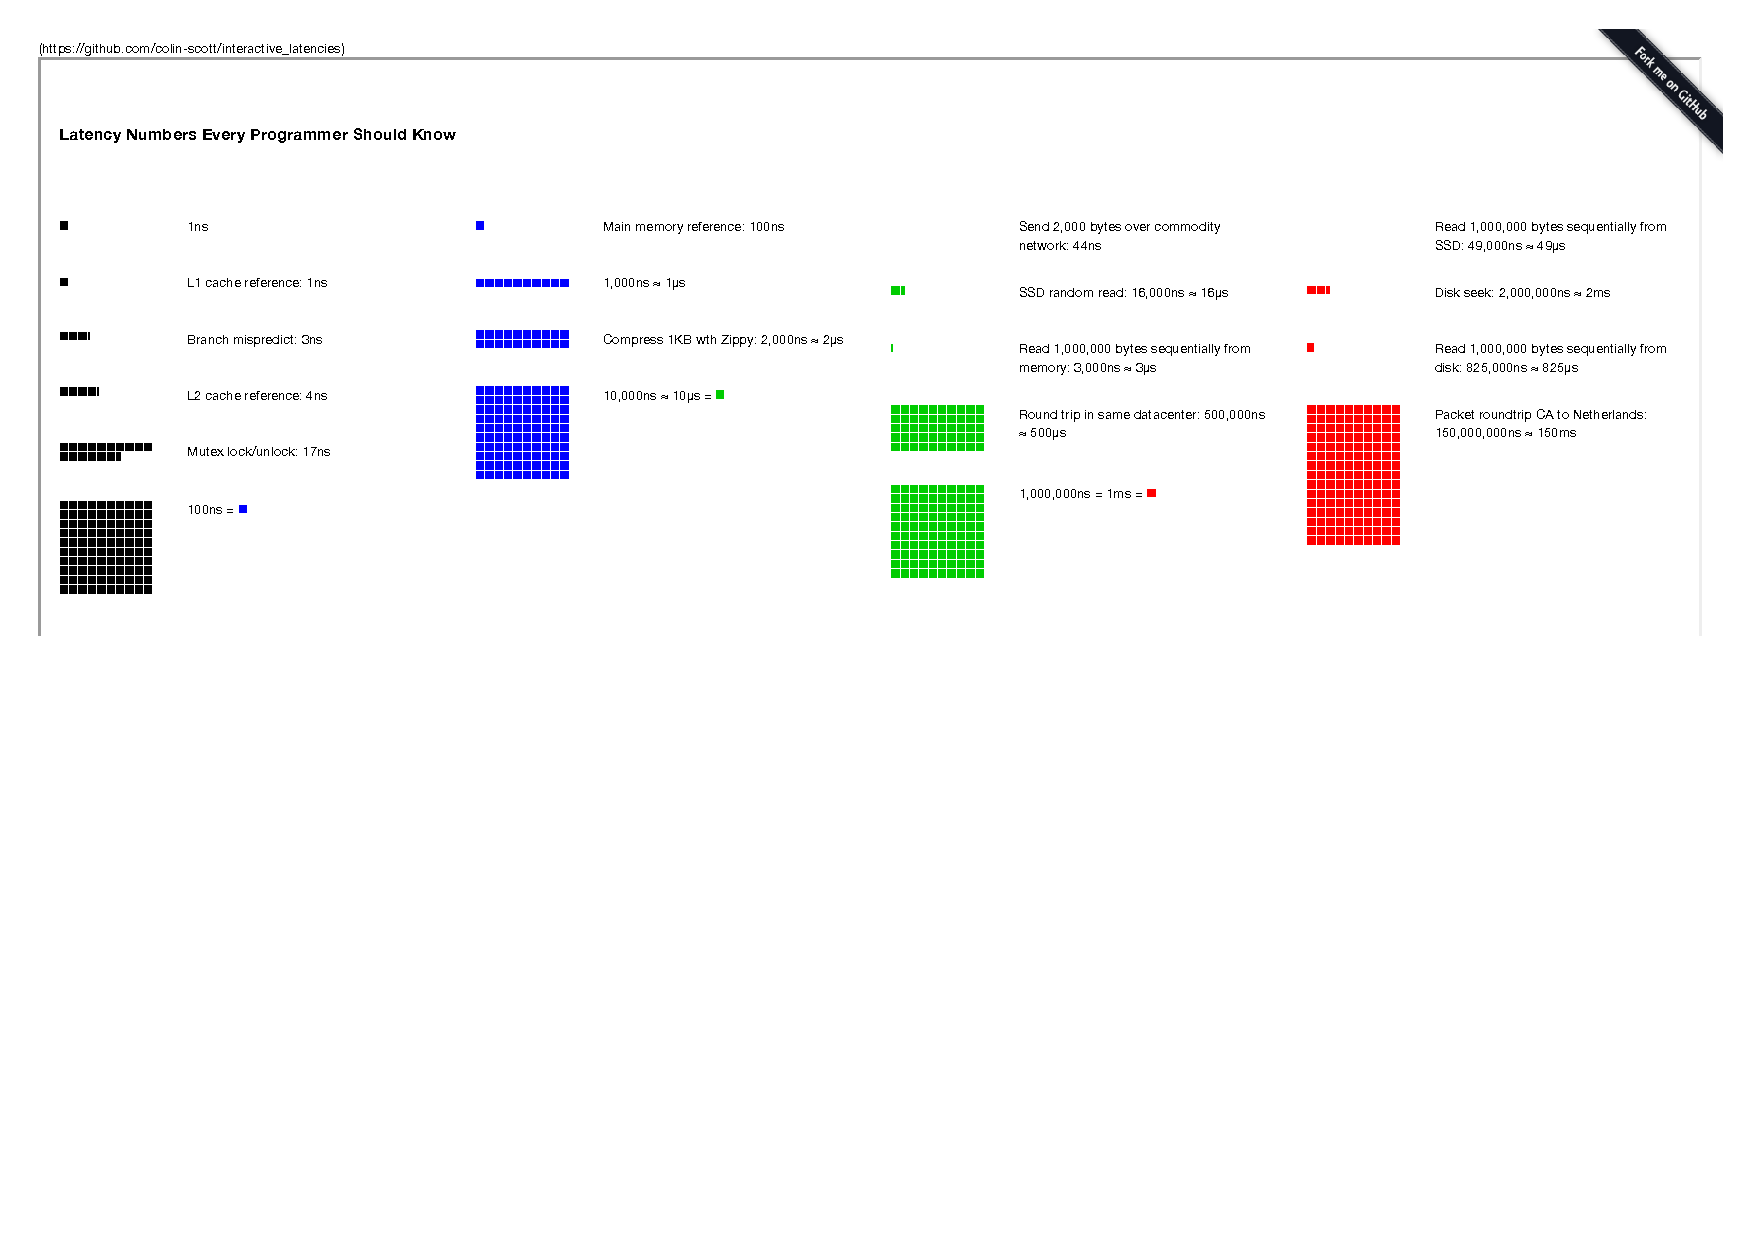
\includegraphics[scale = 0.3]{images/Latency_of_Storage_Hierarchy.pdf}
				\caption{存储系统的层次结构}
			\end{minipage}
		\end{figure}
		\item 主存储器的技术指标
		\begin{enumerate}
			\item 存储容量:一个存储器中存储单元的总数,一般用字数(W)或字节数(B)表示
			\item 存取时间:存储器访问时间,指一次读操作命令发出到该操作完成,将数据送到数据总线上所经历的时间。\textit{写操作时间通常等于读操作时间}
			\item 存储周期:连续两次读写操作所需的最小间隔时间。\textit{存储周期一般大于存取时间}
			\item 存储器带宽:单位时间内存储器存取的信息量,用字/秒、字节/秒或位/秒表示。是衡量数据传输速率的重要指标,决定了以存储器为中心的计算机系统获得信息的速度,是改善机器性能瓶颈的一个关键因素。提高存储器带宽的措施有:
			\begin{enumerate}
				\item 缩短存取时间、存储周期
				\item 增加存储字长,使每个存取周期可读写更多二进制位数
				\item 增加存储体:存储容量的扩展。 位扩展:增加存储器的横向容量即存储字长;字扩展:增加存储器的纵向容量即存储单元的数量
			\end{enumerate}
		\end{enumerate}
		\item 存储器与CPU的链接:\circled{1}\ CPU地址线的低位线与存储芯片的地址线相连,CPU地址线的高位线或用于存储扩展,或用于片选等其他用途;\circled{2}\ 数据线应当位数一样,否则位扩展存储芯片;\circled{3}\ CPU的读/写命令线一般可以直接连到存储芯片的读/写控制端,通常高电平为读,低电平为写;\circled{4}\ 片选控制信号还与CPU的访存控制信号$\overline{\mathrm{MREQ}}$(低电平有效)有关
		\item cache是全硬件实现,注意和虚存的软件实现相区分。cache只有很少的OS参与量
		\item Cache的写回策略(写命中,不命中还要访存的,分为写时取(调入cache再写)和绕写法(直接写入下一级存储器))。需要和内存进行同步,所以出现了两种方案:\circled{1}\ 写直达:同时写cache和内存,用时为写内存的时间。\circled{2}\ 写回:只有被替换的时候才写回,节约了时间,但是会增加cache的复杂性
		\item 页式虚存
		\begin{figure}[h]
			\centering
			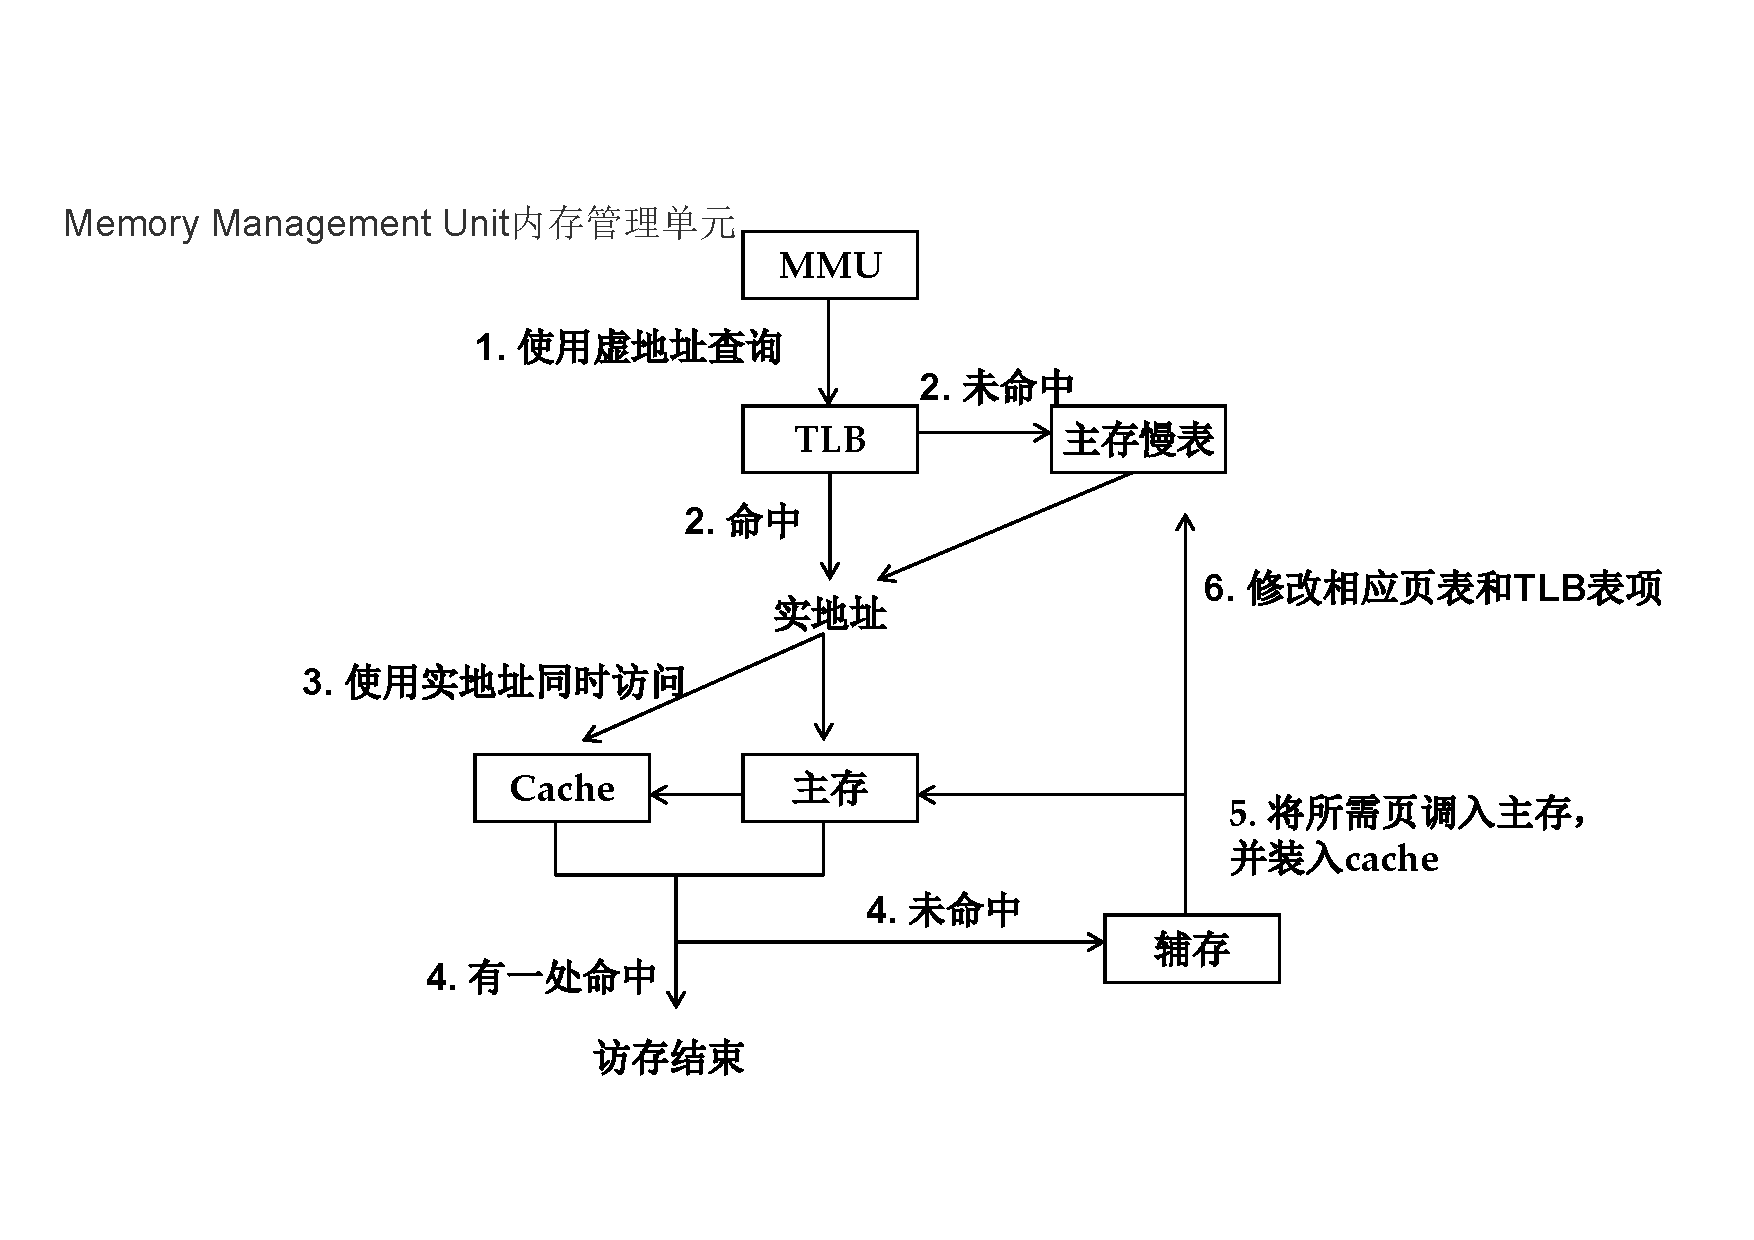
\includegraphics[scale = 0.25]{images/Paging_Virtual_Memory.pdf}
			\caption{页式虚存的访问流程}
		\end{figure}
		\item 总线送入CPU的信号称为输入信号,CPU发出的信号称为输出信号
		\item 总线的性能指标
		\begin{enumerate}
			\item 总线宽度:通常指数据总线的位数
			\item 总线频率:1/传输一次数据时间
			\item 总线带宽:总线的数据传输速率,即单位时间内总线传输数据的位数,通常用每秒传输信息的字节数来衡量(比特率和波特率)
			\item 总线复用:一条信号线上分时传送多种信号
			\item 其他指标:如负载能力、电源电压、总线宽度扩展等
		\end{enumerate}
		\item 总线结构:由4部分构成
		\begin{enumerate}
			\item 数据传送总线:数据、地址、控制
			\item 仲裁总线:包括总线请求线和总线授权线
			\item 中断和同步总线:用于处理带优先级的中断操作,包括中断请求线和中断响应线
			\item 公用线:包括时钟线、电源线、地线、复位线及加电/断电的时序信号线等
		\end{enumerate}
		\item 比特率:单位时间内传送的二进制有效数据的位数,单位为bps;波特率:单位时间内传送的二进制数据的位数,单位为bps
	\end{enumerate}


	\section{另外一个perspective来看待组成原理}
	\subsection{计算机体系结构的8种属性}
		\begin{enumerate}
			\item 数据表示:硬件能直接辨识和操作的数据类型和格式
			\item 寻址方式:最小可寻址单位、寻址方式的种类、地址运算(ch2)
			\item 寄存器组织:操作寄存器、变址寄存器、控制寄存器及专用寄存器的定义、数量和使用规则(ch3、ch4)
			\item 指令系统:机器指令的操作类型、格式、指令间排序和控制机构(ch2、ch3、ch4)
			\item 存储系统:最小编址单位、编址方式、主存容量、最大可编址空间(ch6)
			\item 输入输出结构:输入输出的连接方式、处理机/存储器与输入输出设备间的数据交换方式、 数据交换过程的控制(ch7、ch8)
			\item 中断机构:中断类型、中断级别,以及中断响应方式等(ch5)
			\item 信息保护:信息保护方式、硬件信息保护机制
		\end{enumerate}\par
	\subsection{计算机系统概论}
		\begin{enumerate}
			\item 指令和数据都存储于存储器中,计算机如何区分它们?
			\item 综述计算机技术的发展历程及热点问题
			\item 最新Intel处理器的性能指标?
			\item 计算机的开机过程?
			\item C语言计算机模型?
			\item \verb|getchar()| 的实现过程?
			\item PC系统活动与性能分析
			\begin{enumerate}
				\item 跑一个Benchmark,给出结果?每次执行同一个程序,结果都一样?
				\item 主频与计算性能的关系?
			\end{enumerate}
		\end{enumerate}
	\subsection{关于指令系统}
		\begin{enumerate}
			\item CPU的ISA要定义哪些内容?
			\item 8086为什么要采用段式内存管理模式?
			\item Windows系统中可执行程序的格式?
			\item 调研现在常用的处理器是大尾端还是小尾端,如 x86,ARM,MIPS,PowerPC等?
		\end{enumerate}
	\subsection{关于几种CPU的设计}
		\textit{众所周知,组成原理实验是让设计}CPU\textit{的,所以也可以说这门课是围绕着}CPU\textit{来看的(中断和}memory\textit{都在}CPU\textit{里面),总线和外设也是由}CPU\textit{来处理的}
		\begin{figure}[h]
			\centering
			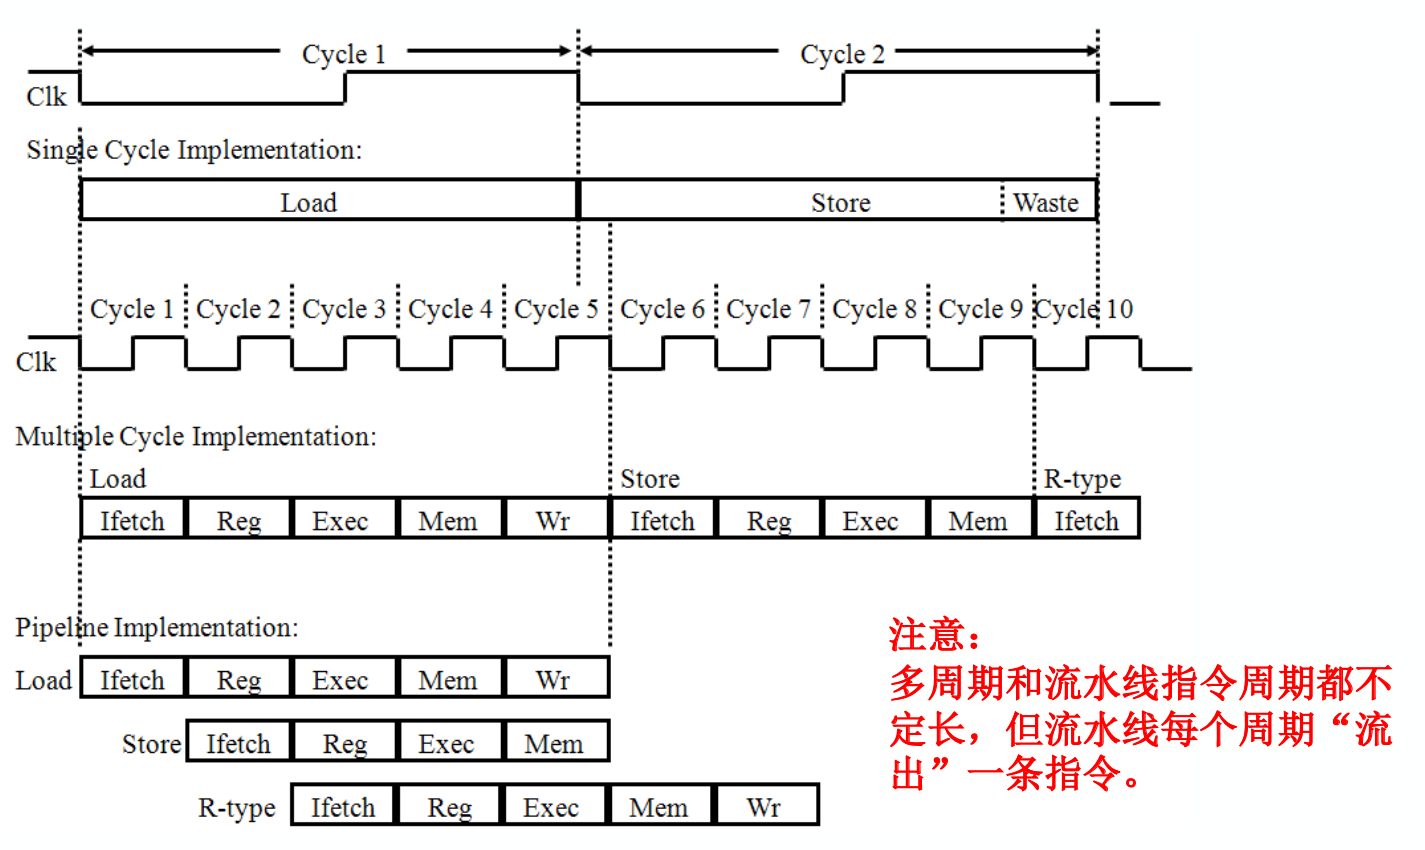
\includegraphics[scale = 0.23]{images/CPU_method.png}
			\caption{SingleCycle, MultiCycle and Pipeline CPU Design}
		\end{figure}
		\begin{enumerate}
			\item 单周期和流水线的关系?
			\begin{quote}
				流水线的控制信号主要继承了单周期的
			\end{quote}
			\item 流水线中实现一个周期访存(取指,取数)的前提条件是什么?
			\item 流水线执行第一条指令时,IF在取指,其他段在做什么?
			\begin{quote}
				如果控制信号清0,则都在执行 \verb|nop| 指令,如果没有清0,由于控制信号未知则……
			\end{quote}
			\item 各流水段的控制信号何时生成与释放?
			\begin{quote}
				都在本指令的ID段生成,在用到的时候从段间寄存器取出
			\end{quote}
			\item 寻址方式如何实现的?哪些寻址方式适合流水线?
			\begin{quote}
				对寄存器堆的访问是在ID段由段间寄存器IR取出\verb|rs = [21:25], rt = [16:20]|得到的寄存器编号,对寄存器进行读操作。隐含寻址(PC)、相对寻址(跳转)、基址寻址(访存)
			\end{quote}
			\item 如果R-type指令也可访存,则应如何设计流水线?
			\item MIPS能否采用“取指、译码、执行”三段流水线?
			\item Stall原因与判断规则?如何实现stall?
		\end{enumerate}
	\subsection{中断系统}
		\begin{enumerate}
			\item 中断周期要完成哪些微操作?
			\begin{quote}
				响应中断、存断点、保存现场、设置屏蔽字、关中断以及跳转ISR
			\end{quote}
			\item 多周期状态机中,出现溢出的指令是否将错误结果写回?
			\begin{quote}
				有可能会,也有可能不会
			\end{quote}
			\item 多周期中状态机中,如何响应中断?
			\begin{quote}
				当前指令周期结束之后响应(下一次IF之前)
			\end{quote}
			\item 指令顺序执行,中断“精确”;指令流水执行,中断“精确”或“非精确”可选
			\item 精确中断,为何提交点是M段?
			\item EPC和cause应该在哪个段?异常检测电路?
			\item mips异常返回指令eret如何实现?
			\item 异常与中断同时发生,优先级?
			\item (分支) 延迟槽中的指令发生异常,EPC = ?
			\item 比较中断、异常、过程调用 (请求时间、响应时间,断点与现场,返回点,同步异步,中断周期、系统状态)
		\end{enumerate}
	\subsection{存储系统}
		\begin{enumerate}
			\item 理解“码距”
			\begin{enumerate}
				\item 具有1位纠错能力的编码系统最小码距是多少?
				\item 单纠错海明码码距是多少?
				\item (n+k, n)CRC码码距是多少?
			\end{enumerate}
			\item 比较海明码与CRC码的容错能力
		\end{enumerate}

	\section{几个比较复杂的points}
	\subsection{寻址}
		指令寻址比较简单,就PC+4或者计算跳跃地址。数据寻址,就是把操作数的形式地址A,通过寻址特征,变换为操作数的有效地址EA的过程\par
		\begin{table}[h]
			\centering
			\begin{tabular}{cccc}
				\toprule
				&Algorithms&Main Merits&Main Drawbacks\\
				\midrule
				隐含寻址&操作数在专用寄存器&无存储器访问&数据范围有限\\
				立即寻址&地址段直接存立即数&无存储器访问&操作数幅值有限\\
				直接寻址&EA=A&简单&地址范围有限\\
				间接寻址&EA=(A)\footnote{括号意为访存结果}&大的地址范围&多重存储器访问\\
				寄存器寻址&EA=R&无存储器访问&地址范围有限\\
				寄存器间接寻址&EA=(R)&大的地址范围&额外存储器访问\\
				偏移寻址&EA=A+(R)&灵活&复杂\\
				段寻址(偏移)&EA=A+(R)&灵活&复杂\\
				堆栈寻址&EA=栈顶&无存储器访问&应用有限\\
				\bottomrule
			\end{tabular}
		\end{table}\par
		\textit{下面以MIPS指令集为例解释一下这些寻址方式的一部分,没写的就是没有对应的例子:}\par
		\begin{enumerate}
			\item 隐含寻址:指令中不明显给出操作数的地址,而是隐含在特定的寄存器中,有利于缩短指令字长
			\item 立即寻址:指令的地址字段指出的不是操作数地址,而是操作数本身。取出指令就可同时获得操作数,不必访问内存\ \verb|addi|
			\item 直接寻址:形式地址即为真实地址\ \verb|jump|
			\item 间接寻址:访存来解锁下一步线索/地址。另一个优点是便于编程,尤其是调用函数返回的时候,调用子程序前,将返回地址存入子程序最末条指令的形式地址的存储单元,便可准确返回原程序,如图所示\dag\footnote{附图均在本节最后}
			\item 寄存器寻址:取出寄存器内部的数据\ \verb|对rs,rt的访问|
			\item 寄存器间接寻址
			\item 偏移寻址:看下面的mindnode\ddag (注释一下段寻址方式:将主存空间分为若干段,每段的首地址存于基址寄存器,段内偏移量由指令字中的形式地址A指出)
			\item 相对寻址:偏移寻址的一种,偏移量常用补码表示,基于局部性原理
			\item 堆栈寻址
		\end{enumerate}\par
		\begin{figure}[h]
			\centering
			\begin{minipage}{20em}
				\centering
				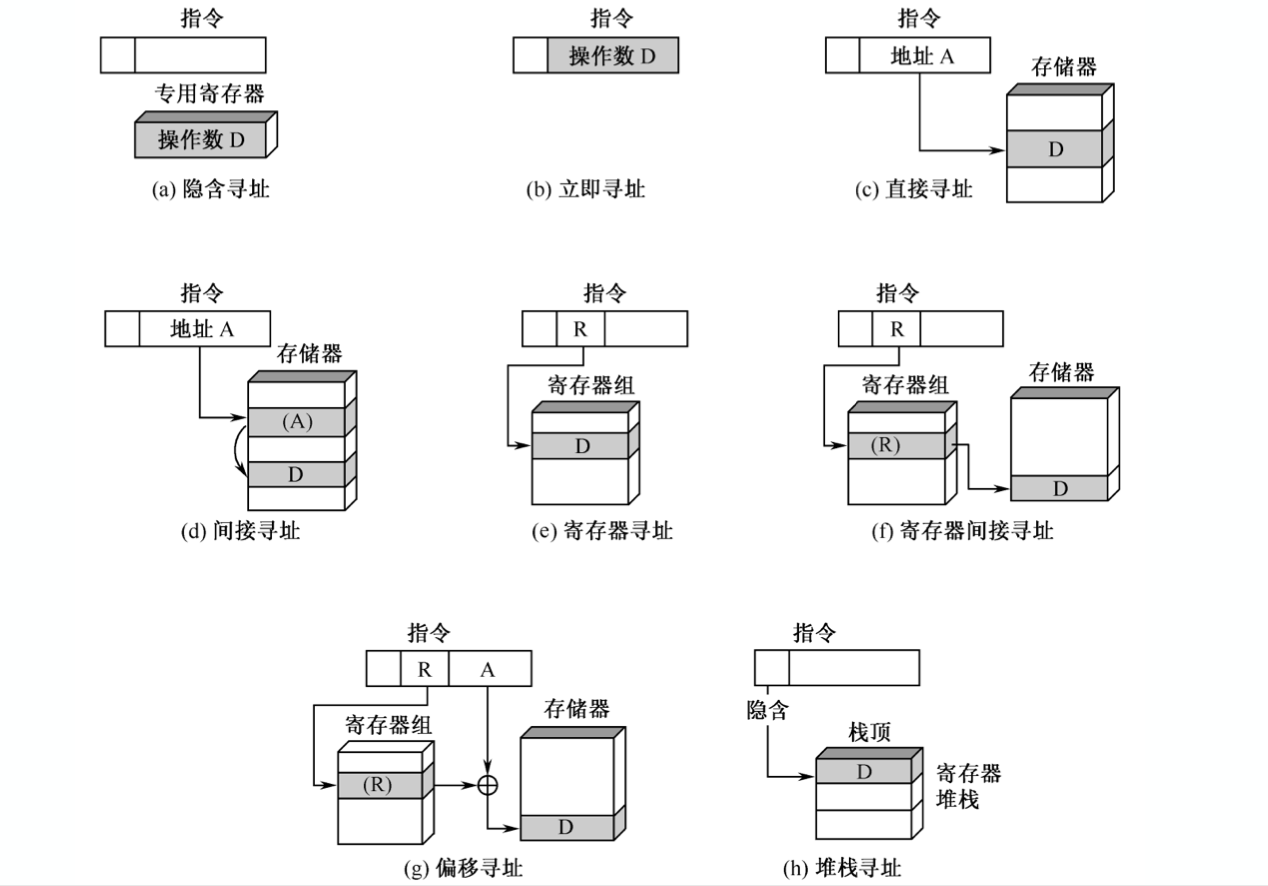
\includegraphics[scale = 0.12]{images/memory_visiting.png}
				\caption{Big Picture}
			\end{minipage}
			\qquad
			\begin{minipage}{20em}
				\centering
				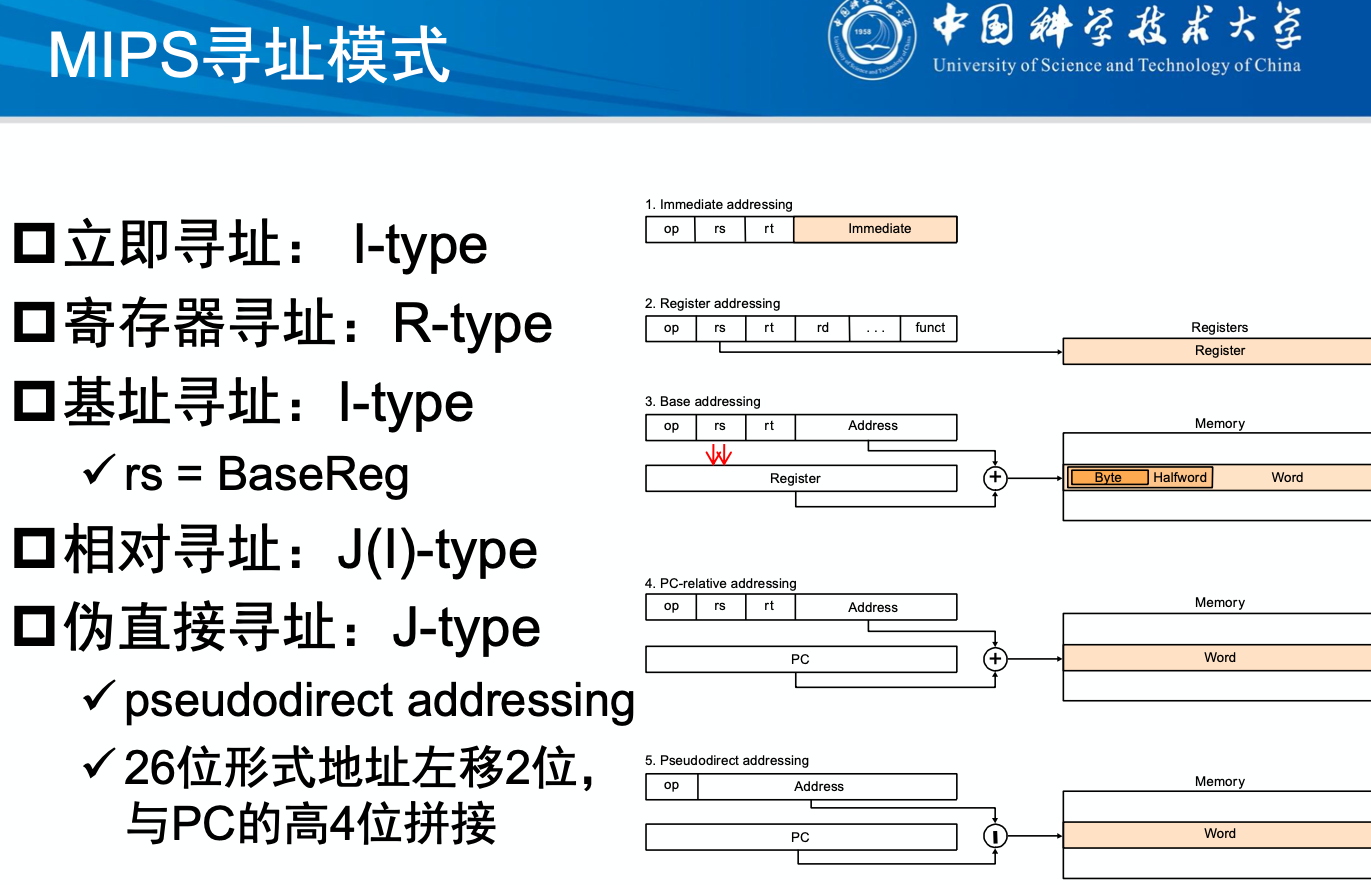
\includegraphics[scale = 0.12]{images/MIPS_addr_seek.png}
				\caption{MIPS Address}
			\end{minipage}
		\end{figure}\par
		\textit{对基址寻址和变址寻址的对比,其实我觉得记住}\verb|lw|\textit{是基址寻址就}OK。
		\begin{enumerate}
			\item 基址寻址(Base or Displacement addressing)
			\begin{enumerate}
				\item 以基址寄存器(BR)为基准进行寻址
				\item EA = 形式地址 + BR
				\item 基址寄存器:专用、通用 (显式(通用寄存器)、隐式(专用寄存器))
			\end{enumerate}
			\item 变址寻址(index)
			\begin{enumerate}
				\item 以变址寄存器(IX)的值为基准寻址
				\item EA = 形式地址 + IX
				\item 变址寄存器:专用、通用 (显式(通用寄存器)、隐式(专用寄存器))
			\end{enumerate}
			\item 基址寻址 vs. 变址寻址
			\begin{enumerate}
				\item 基址:BR由OS赋值,不变;形式地址可变
				\item 变址:IX由程序员赋值,可变;形式地址不变
				\item 用途不同:基址—段寻址,变址—数组、字符串、循环
			\end{enumerate}
			\item 基址寄存器是一个很长的寄存器,因为需要访问到所有的内存空间,才能给出每一个段的首地址
			\item 变址寻址多数用在循环或者数组的自增操作上,所以IX寄存器不需要特别大
			\item 从实现的角度来讲,也就是寄存器名字,叫成BR还是IX,并开对应WIDTH
			\item 由于虚拟内存的地址映射,进程在调用地址空间时是一块连续的memory,故基址寻址偏移不会 segmentation fault。BR是在OS创建进程的时候,调进去的,所以说是由OS管理
		\end{enumerate}
		\begin{figure}[h]
			\centering
			\begin{minipage}{20em}
				\centering
				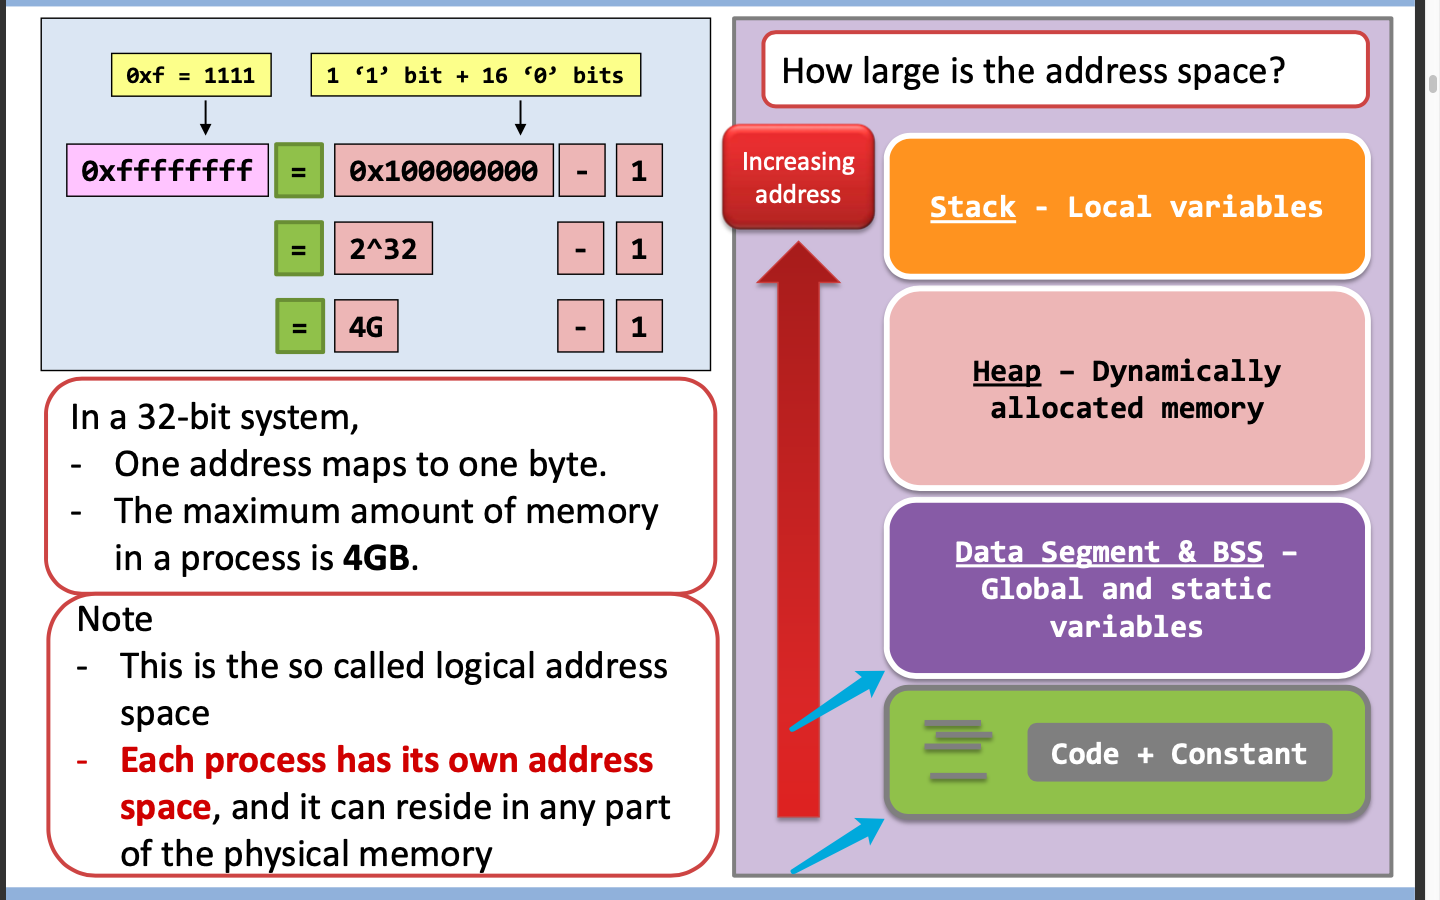
\includegraphics[scale = 0.12]{images/Data_Segment_of_Process.png}
				\caption{Data Segment (quoted from OS)}
			\end{minipage}
			\qquad
			\begin{minipage}{20em}
				\centering
				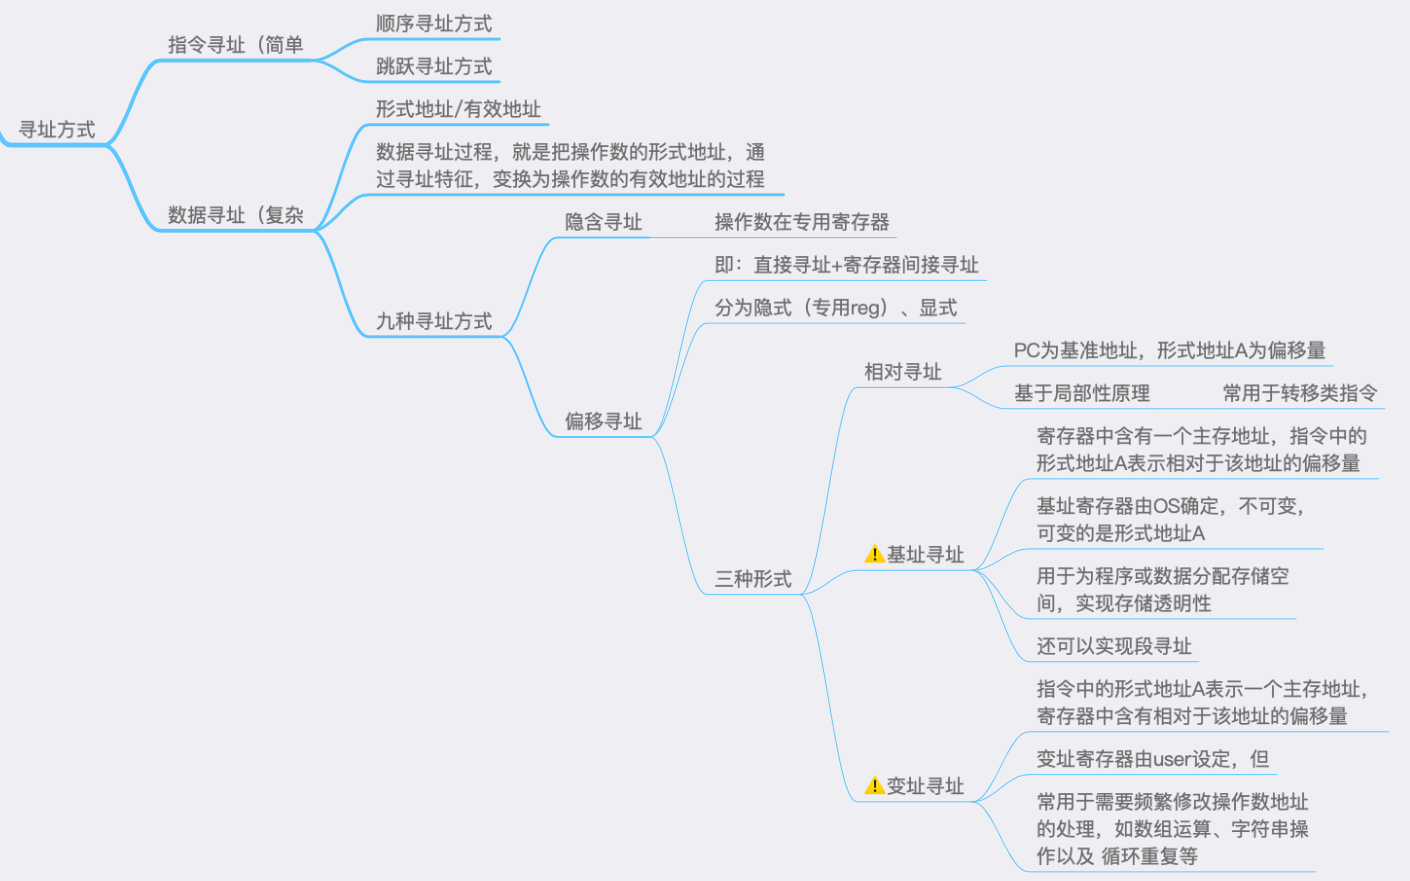
\includegraphics[scale = 0.12]{images/memory_visiting_mindmap.png}
				\caption{\ddag 偏移寻址}
			\end{minipage}
			\\[10pt]
			\begin{minipage}{20em}
				\centering
				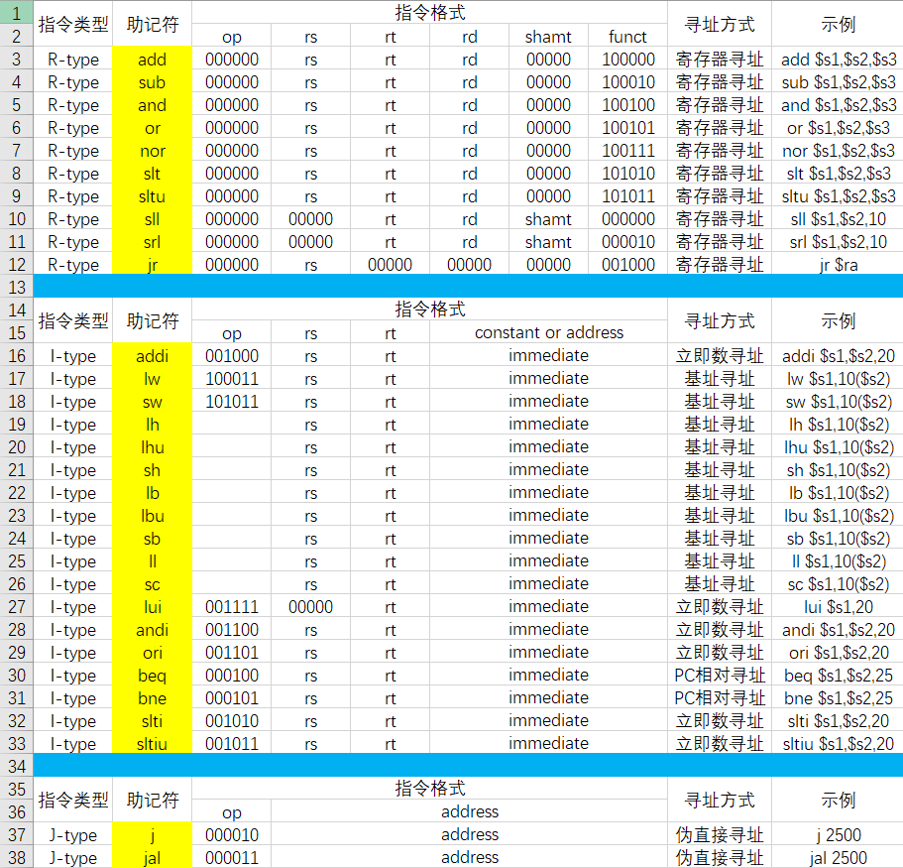
\includegraphics[scale = 0.32]{images/address_seeking_in_MPIS.png}
				\caption{MIPS Address Seek}
			\end{minipage}
			\qquad
			\begin{minipage}{20em}
				\centering
				\begin{minipage}{20em}
					\centering
					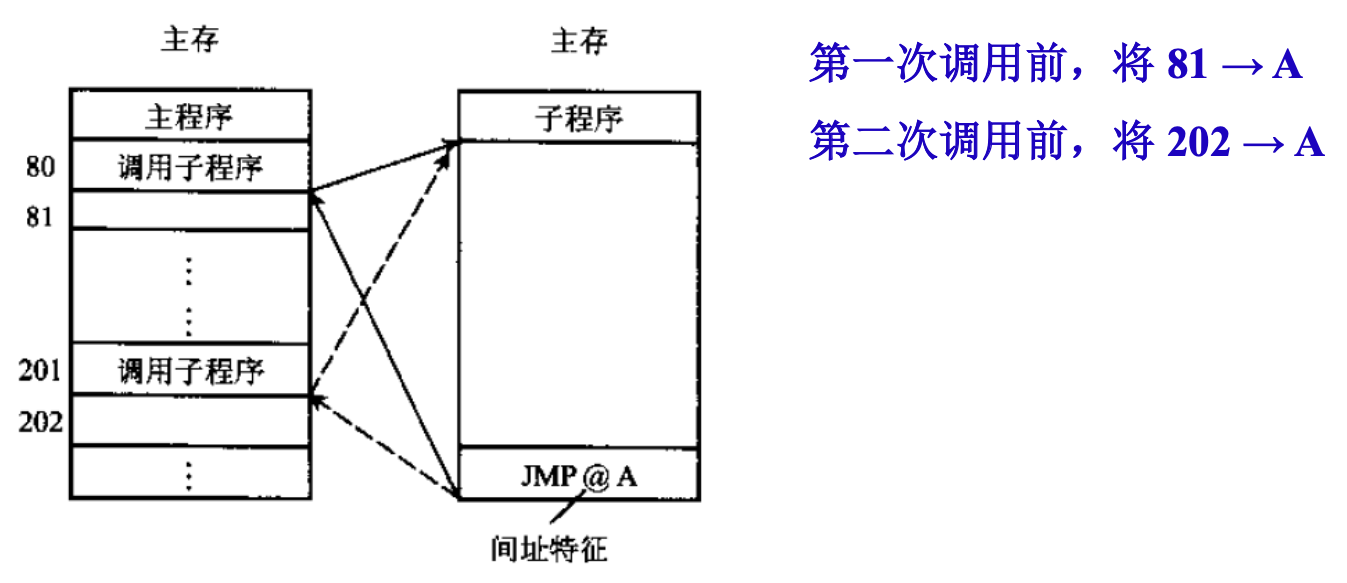
\includegraphics[scale = 0.12]{images/indirect_addressing.png}
					\caption{\dag 间接寻址方式的优点——便于编程}
				\end{minipage}
				\\[7pt]
				\begin{minipage}{20em}
					\centering
					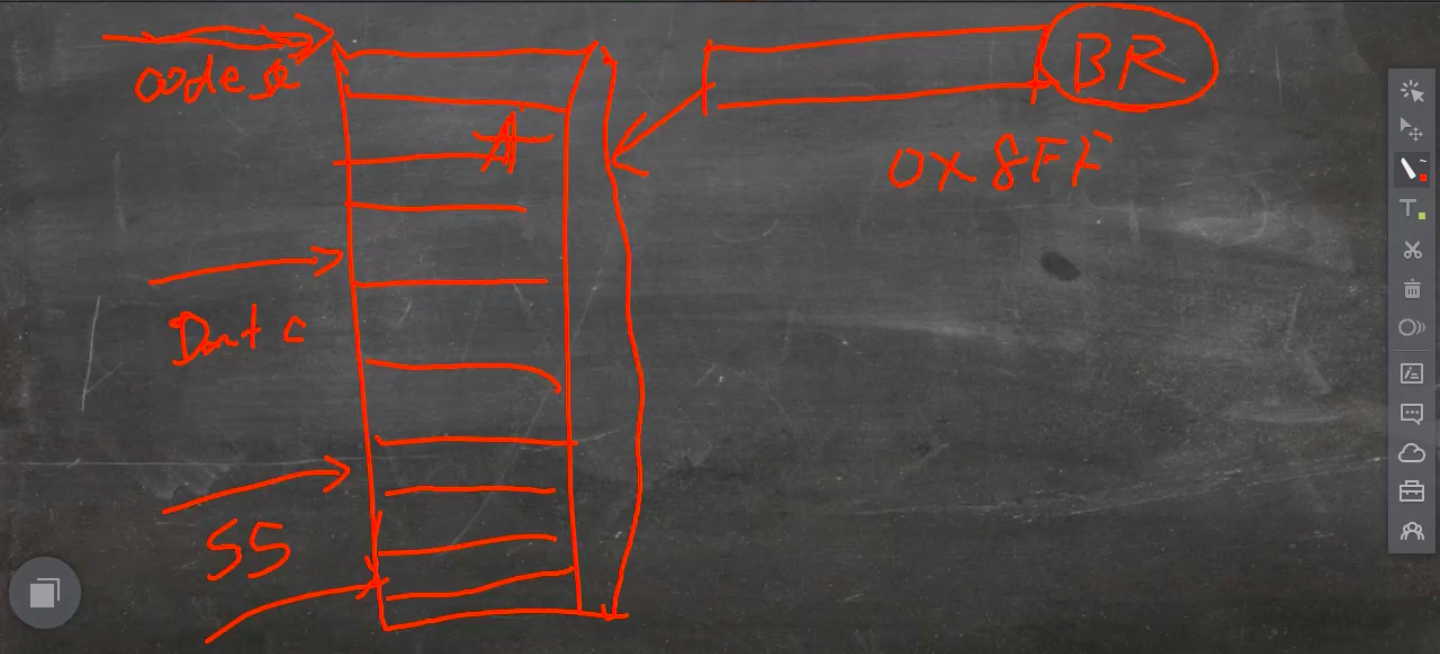
\includegraphics[scale = 0.12]{images/BR_and_Data_Segment.png}
					\caption{BR and Data Segment}
				\end{minipage}
			\end{minipage}
		\end{figure}\par
	\subsection{中断\&异常(理论)}
		三种中断:Exceptions异常(随时发生,随时处理)、Interrupts中断(随时发生,延迟响应)、Traps陷阱(专用指令,特殊处理)\par\noindent
		\paragraph{中断系统需要解决的问题:}
		\begin{enumerate}[label={\sffamily(\alph{*})}]
			\item 各中断源如何向CPU提出请求 ?(INTR, INTA)
			\item 各中断源同时提出请求怎么办 ? (中断判优-程序查询,硬件排队-集中、分布)
			\item CPU什么条件、什么时间、以什么方式响应中断 ? (指令周期结束,中断隐指令)
			\item 如何保护现场 ?(中断隐指令断点、ISR、堆栈)
			\item 如何寻找入口地址 ?(硬件向量,软件查询)
			\item 如何恢复现场,如何返回 ?(中断隐指令断点、ISR、堆栈)
			\item 处理中断的过程中又出现新的中断怎么办 ? (多重中断,可屏蔽,设置屏蔽字)
		\end{enumerate}
		\paragraph{中断机构组成}
		\begin{enumerate}
			\item CPU中断禁止/允许:IF@PSW。PSW即程序状态字(程序状态寄存器),Program Status Word。
			\begin{figure}[h]
				\centering
				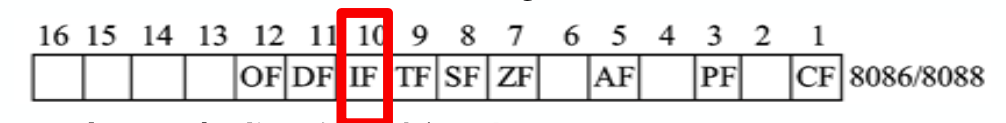
\includegraphics[scale = 0.2]{images/IF_PSW.png}
			\end{figure}
			\item CPU中断请求/响应控制:INTR、INTA
			\item 中断响应/返回:中断隐指令
			\item 断点/现场保存:MEM(stack)
			\item 中断服务 \circled{1}\  中断源识别/判优:中断控制器\ \circled{2}\  ISR (Interrupt Service Routine)入口:向量方式、非向量方式
		\end{enumerate}
		\paragraph{中断请求标记 INTR}\texttt{\textit{(各中断源如何向CPU提出请求?)}}
		一个请求源对应一个INTR中断请求标记触发器,多个INTR组成中断请求标记寄存器。ITR可以分散在各个中断源的接口电路里面或者集中在CPU的中断系统内部。INTR (interrupt request) 和 INTA (interrupt acknowledge) 都是控制信号
		\paragraph{中断判优逻辑}\texttt{\textit{(各中断源同时提出请求怎么办?)}}\verb|if-else| 优先级
		\begin{enumerate}
			\item 软件实现(程序查询)
			\item 硬件实现(排队器),分为\ \circled{1}\  分散在各个中断源的接口电路中的链式排队器\ \circled{2}\  集中在CPU内的链式排队器
		\end{enumerate}
		\paragraph{中断响应}\texttt{\textit{(CPU在什么条件、什么时间、以什么方式响应中断?)(如何寻找入口地址?)}}
			\subparagraph{响应中断的条件} CPU允许中断触发器 \verb|EINT == 1|
			\subparagraph{响应中断的时间} \textit{指令执行周期结束时刻由CPU发查询信号}
			\begin{enumerate}
				\item 外部中断(IO):异步(延迟响应),指令周期结束
				\item 内部中断(陷阱和异常):同步(“马上”响应)
			\end{enumerate} \indent\textbf{注意一个指令周期可能包含多个时钟周期}
			\subparagraph{中断隐指令} \textit{中断周期完成的主要操作,通过中断隐指令完成}
			\begin{enumerate}
				\item 保护程序断点\footnote{断点仅指PC,或者NPC}:断点存于特定地址(如0号地址)内,或者在堆栈
				\item 寻找服务程序入口地址:
				\begin{enumerate}
					\item 向量地址 $\to$ PC(硬件向量法):在ISR里面有很多 \verb|JMP| 跳转到特定的内存空间,排队器输出到向量地址形成部件里面,然后间接访存跳转到ISR的入口地址(把入口地址哈希起来是一个连续数组可以提高性能?(雾))
					\item 中断识别程序入口地址M $\to$ PC(软件查询法)
				\end{enumerate}
				\item 硬件关中断(其实也可以不做,实现嵌套中断):\circled{1}\ ENIT允许中断触发器置为0\ \circled{2}\ INT中断标记触发器置为1
			\end{enumerate}
			\subparagraph{中断周期} \textit{由于中断的延迟响应特性,在CPU写回之后才会着手查询和响应可能出现的Interrupts。}中断即CPU与中断控制器通信,响应外部事件(INTR,INTA),包括\  \circled{1}\  是否有中断请求\ \circled{2}\  识别中断源,获得中断向量。采取的动作:存PC和PSW,关中断,转ISR
		\paragraph{保护和恢复现场}\texttt{\textit{(如何保护现场?)(如何恢复现场、如何返回?)}}保护现场分为断点和寄存器内容两部分。前者由中断隐指令,通过压栈\footnote{栈的地址由高向低生长(OS)}或者存在特定地址完成;后者由ISR压栈完成,是一个被调用者保存策略,只需保存部分寄存器(ISR中可能还会涉及关中断和开中断,(参考OS里面critical section should be as tight as possible的说法,)在保护现场两端需要关掉中断)。恢复就是反过来,返回是从栈里面再读出来PC值(为什么不用间接寻址?)
		\paragraph{中断屏蔽技术}\texttt{\textit{(处理中断的过程中又出现新的中断怎么办?)}}
		\subparagraph{多重中断的概念} 中断嵌套,即在执行ISR的过程中出现并响应了新的中断请求,亦即中断服务函数的嵌套调用
		\subparagraph{实现多重中断的条件}
		\begin{enumerate}
			\item 提前设置开中断,即中断隐指令响应,存断点之后关中断;中断服务开始之后(保护现场结束之后,ISR核心程序开始之前)开中断。以及在恢复现场之前关中断,之后开中断
			\item 优先级别高的中断源有权中断优先级别低的中断源
		\end{enumerate}
		\subparagraph{屏蔽技术}
		\begin{enumerate}[label = \circled{\arabic{*}}]
			\item 屏蔽触发器的作用:动态优先级设定,若某高优先级的中断源其MASK$_i$ 为1,则它的请求将被屏蔽,即手动调整它的优先级为无穷低
			\item 屏蔽字:每一个中断源都在ISR中有自己的屏蔽字(姑且称为 $\vec{x}_i$ ),其位数均等于中断源总数。若 $\vec{x}_i$ 的第 $m$ 项为0,则中断源$i$不能屏蔽中断源 $m$。
			\item 新屏蔽字的设置:新的中断服务流程为:保护现场 - 置屏蔽字 - 开中断 - 中断服务 - 关中断 - 恢复现场 - 恢复屏蔽字 - 开中断
			\item 屏蔽技术可以改变处理的优先等级(响应优先级不可改变;处理优先级可改变(通过重新设置屏蔽字))\newline
			\begin{figure}[h]
				\centering
				\begin{minipage}{20em}
					\centering
					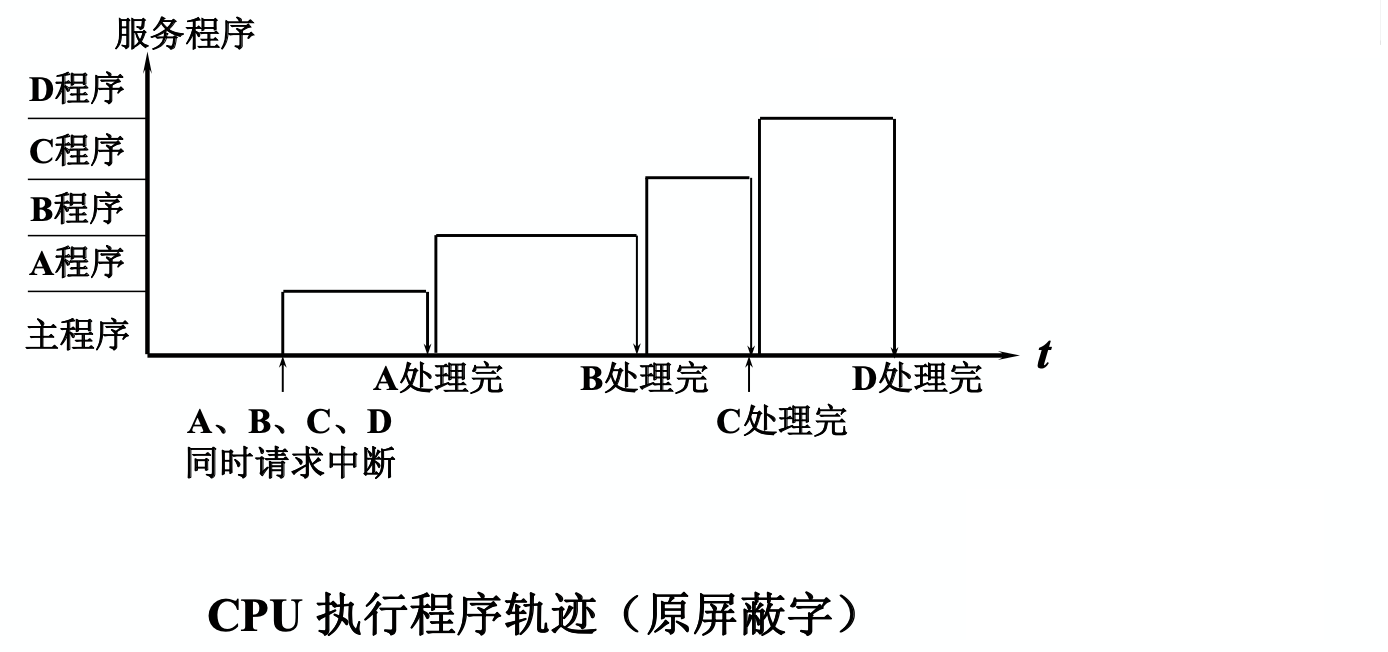
\includegraphics[scale = 0.12]{images/ISR_Original.png}
					\caption{响应优先级即处理优先级}
				\end{minipage}
				\qquad
				\begin{minipage}{20em}
					\centering
					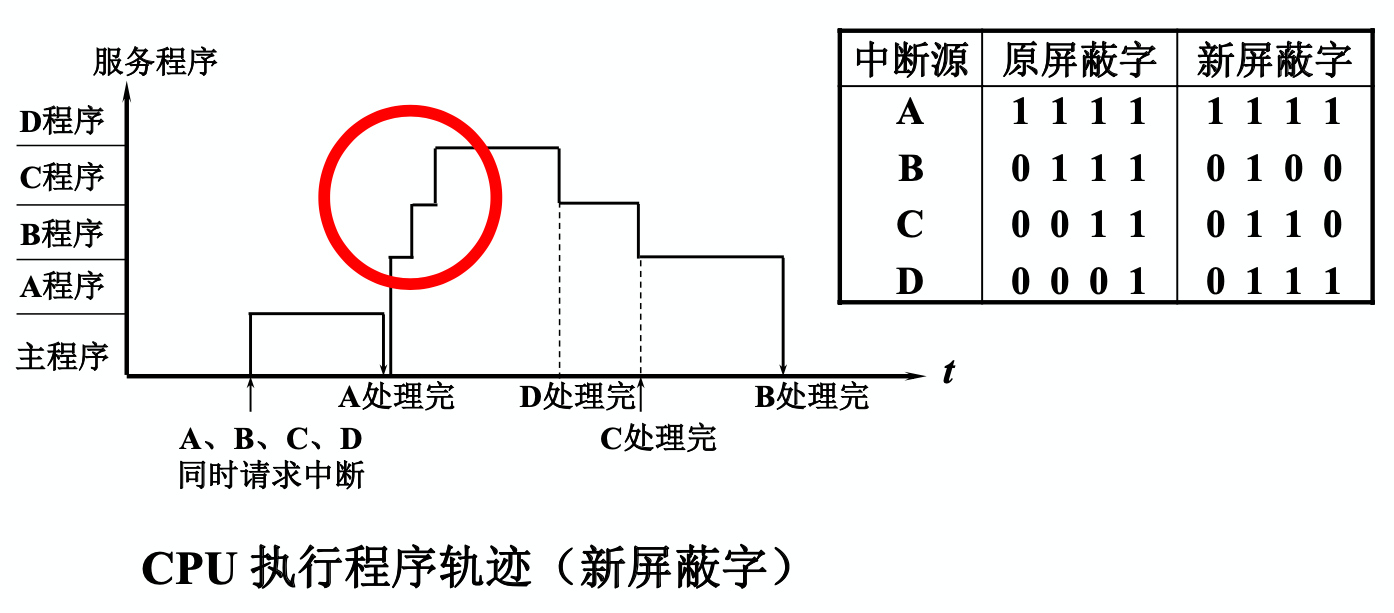
\includegraphics[scale = 0.12]{images/ISR_Masked.png}
					\caption{响应后不一定处理}
				\end{minipage}
			\end{figure}
			新屏蔽字图中,红色圈里面的锯齿为BCD三个中断请求的响应时间(响应时间包括保存断点、保存现场、设置新的屏蔽字)。出现这种情况的原因是响应优先级与处理优先级不一致。由原屏蔽字表每一行0的数量可知,响应优先级 A$\to$B$\to$C$\to$D 降序排列,当响应某一个中断请求(如B)并进入ISR时,置屏蔽字一步会将屏蔽触发器组按照B的新屏蔽字置数,即只有B的请求被屏蔽。在执行ISR时,和以前一样会在WB之后检查中断请求,这时A已经处理完成,B已经响应,C和D正在请求且未被屏蔽,于是按照\textbf{响应优先级}响应C的请求。这样做的目的是可以提供一个人为改变实际处理顺序的机会,让在物理上优先级低的中断源设备也可以先处理更重要的请求,或者人为地屏蔽某个中断源的请求,便于程序控制
		\end{enumerate}
	\subsection{流水线CPU中的异常处理}
		\textit{多周期的比较简单,就只放几个图吧}\newline
		\begin{figure}[h]
			\centering
			\begin{minipage}{20em}
				\centering
				\begin{minipage}{20em}
					\centering
					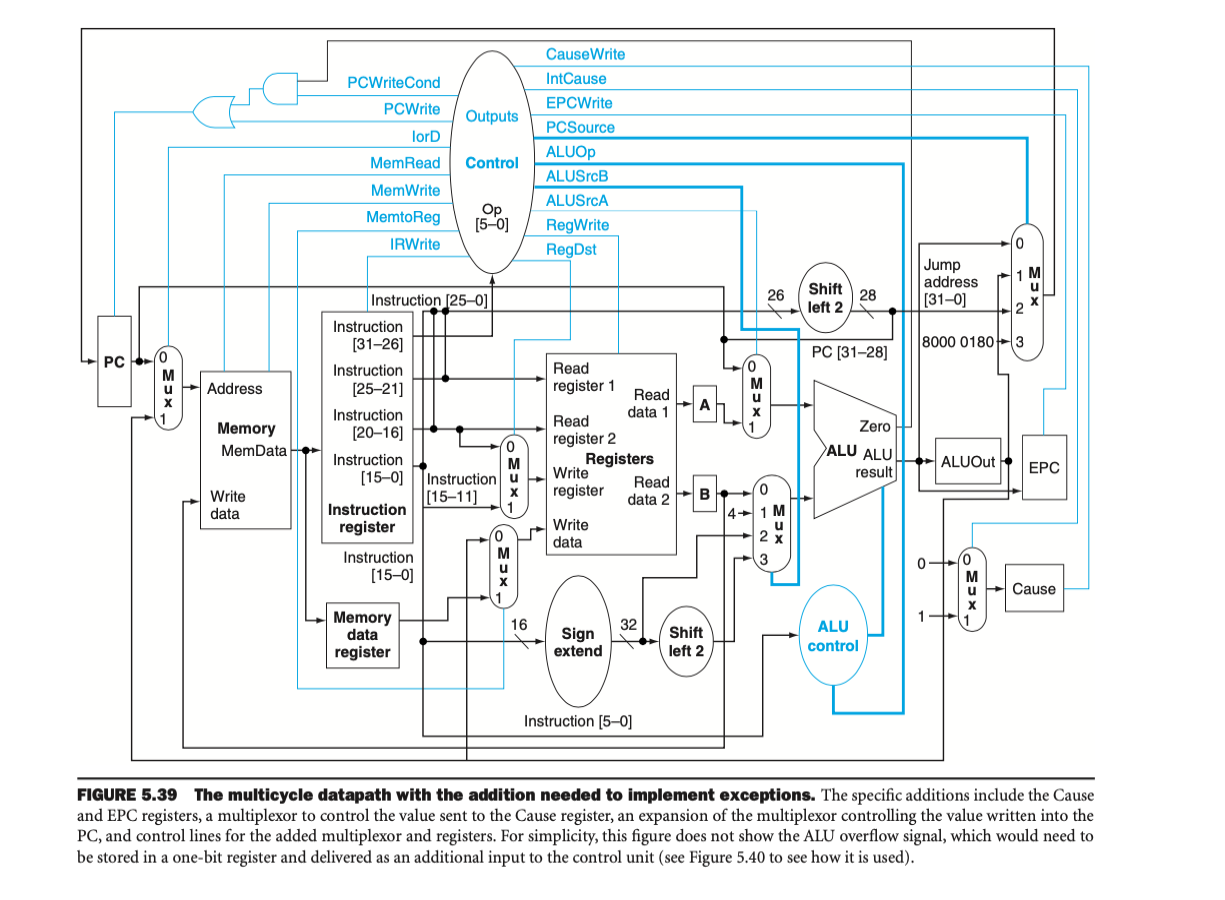
\includegraphics[scale = 0.14]{images/MultiCycle_Exceptions.png}
					\caption{多周期异常处理数据通路}
				\end{minipage}
				\\[10pt]
				\begin{minipage}{20em}
					\centering
					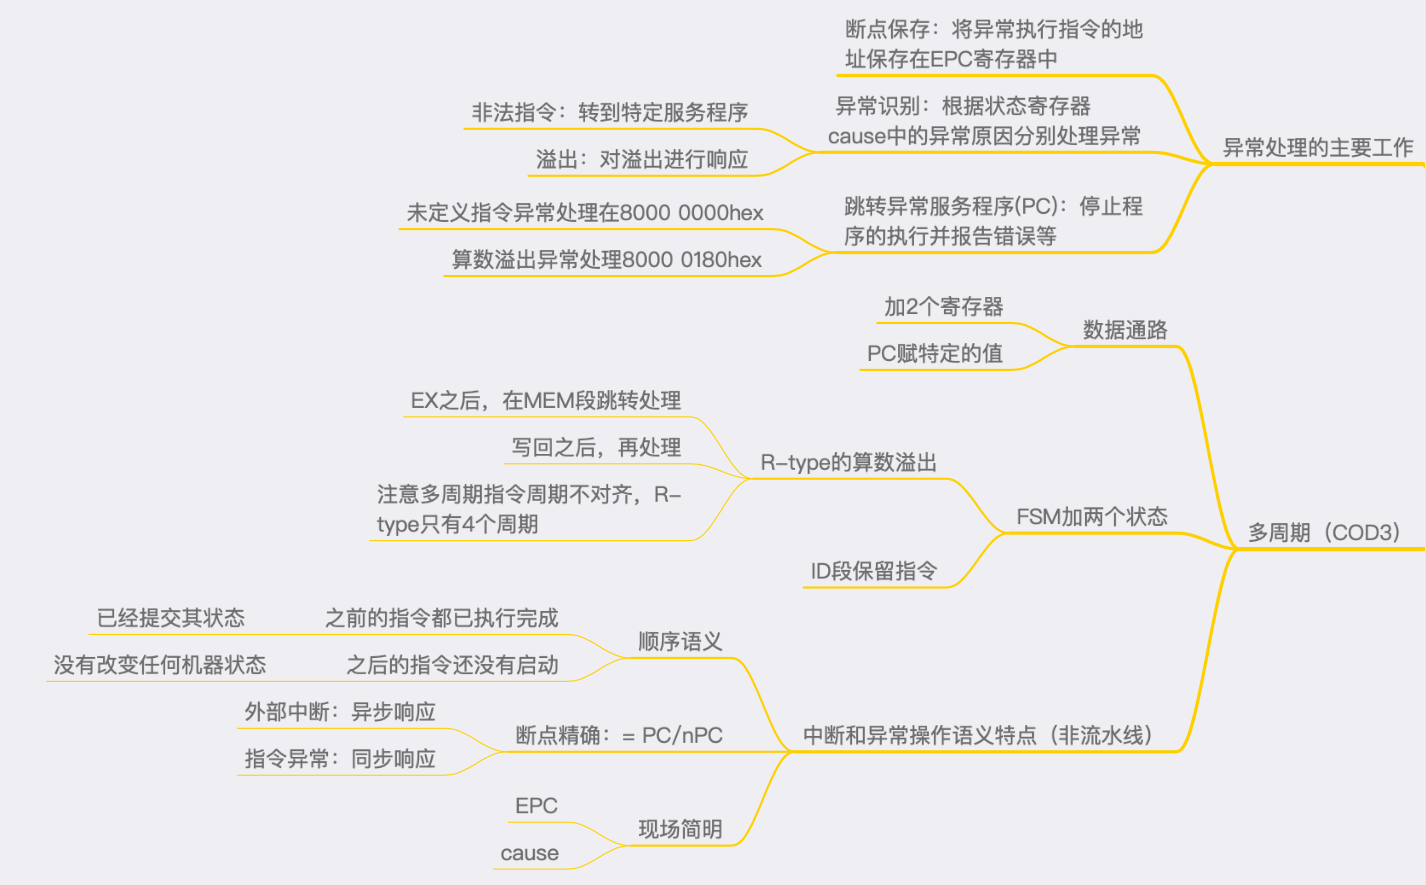
\includegraphics[scale = 0.13]{images/MultiCycle_Exceptions_MindNode.png}
					\caption{多周期异常处理主要内容}
				\end{minipage}
			\end{minipage}
			\qquad
			\begin{minipage}{20em}
				\centering
				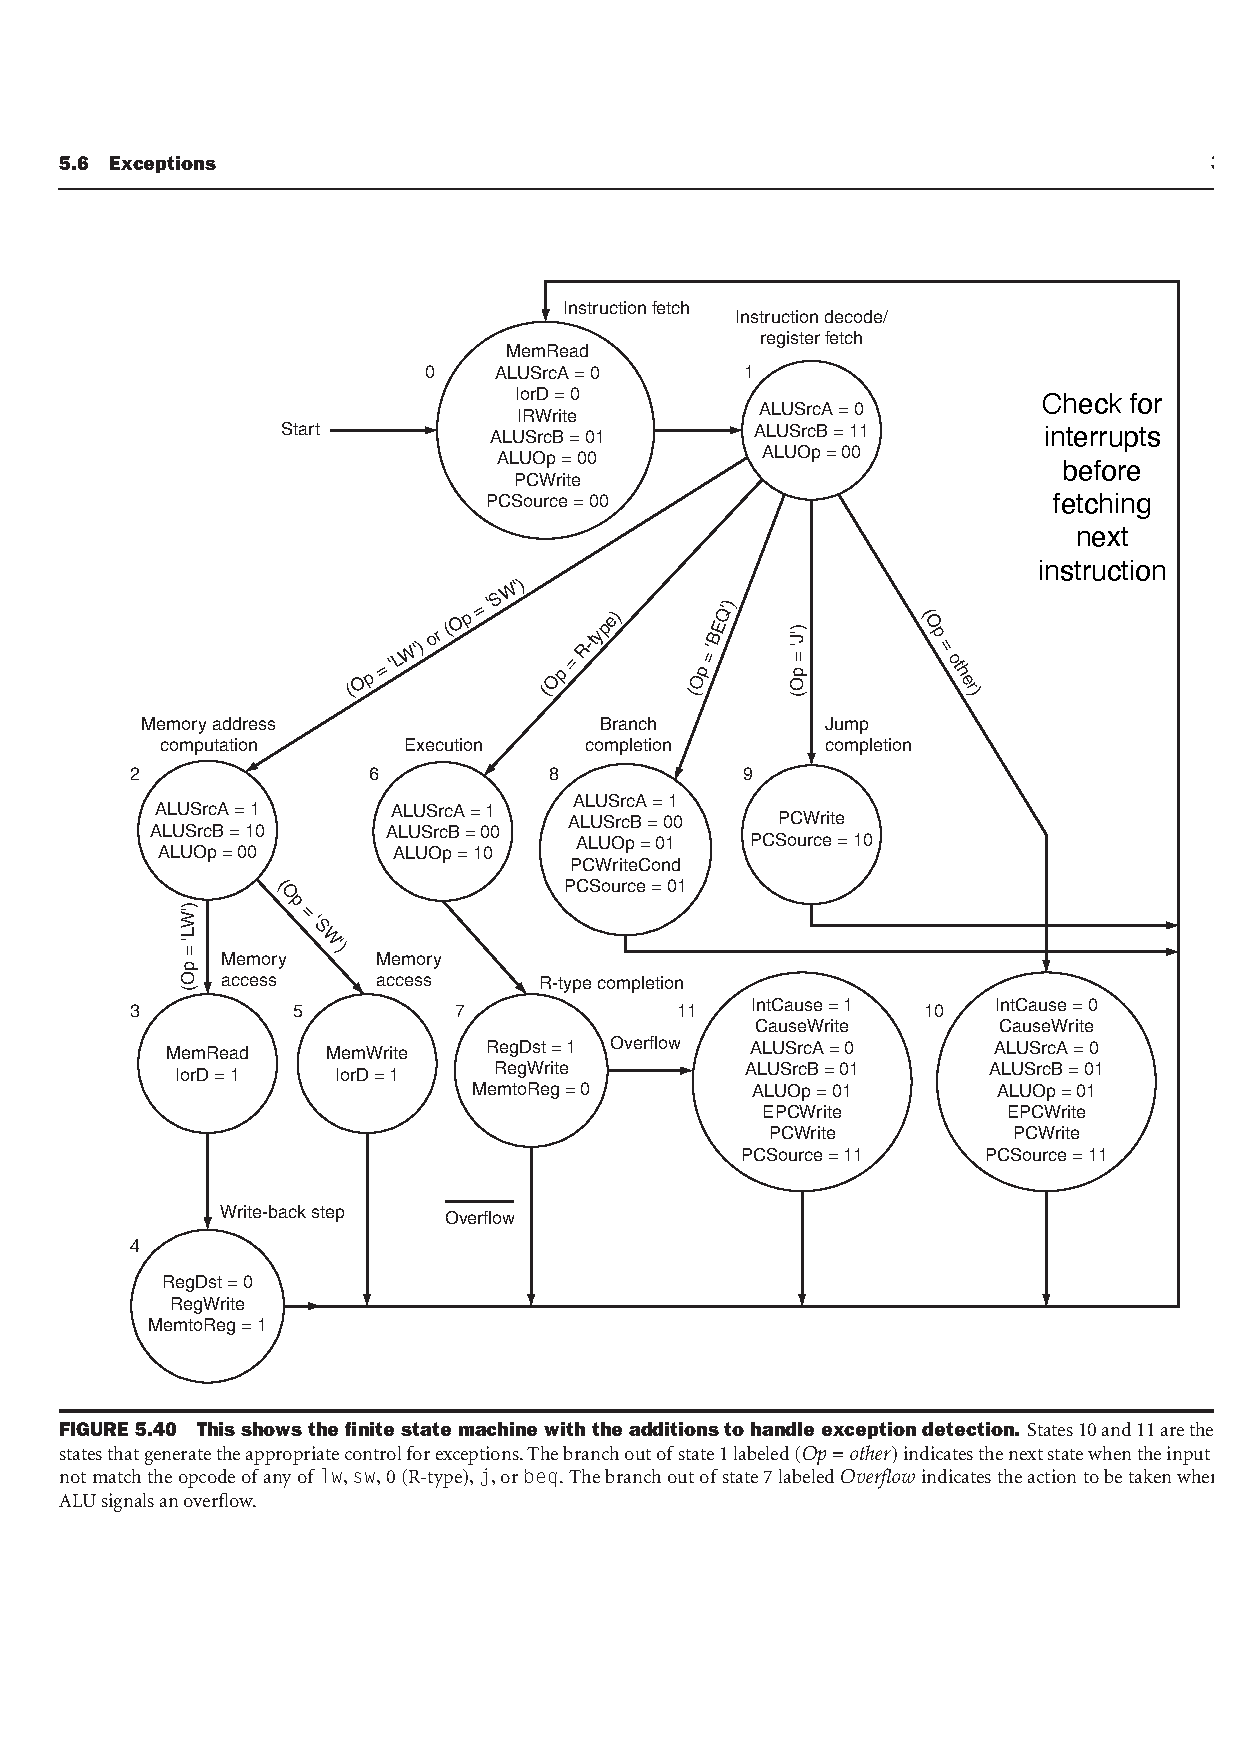
\includegraphics[scale = 0.32]{images/MultiCycle_Exceptions_FSM.pdf}
				\caption{多周期异常处理状态机}
			\end{minipage}
		\end{figure}\par
		流水线的处理较多周期要复杂很多,这是由流水线的并行导致的。在流水线里面,“顺序执行”只是一种逻辑关系:断点和状态难以确定。
		\begin{enumerate}
			\item 后续指令在产生异常指令完成之前改变了系统的部分状态,如 \verb|lw| 指令在MEM段产生异常,而其后的R-type指令设置了0标志(PSW内程序状态字)
			\item 异常发生顺序与指令执行顺序不一定相同,如 \verb|addi| 指令在ID段CC3发生异常,但 \verb|lw| 指令在MEM段CC4异常
			\item 转移指令和分支预测给异常处理带来了麻烦
		\end{enumerate}
		\textbf{流水线处理分为非精确处理和精确处理两种,非精确处理也有简单一些的和复杂一些的}
		\paragraph{非精确方案1:甩锅} \textit{允许已进入流水线中的指令都做完再去做异常处理。}断点:无论在第i条指令的哪一级流水段发生异常,都不再允许后继指令进入流水线,断点为\textbf{最后进入流水线}那条指令的地址(非精确:断点不是当前指令;可变:不同段发生异常,EPC增量不同)。这种方案需要比较强的OS支持,因为没有给出来具体哪一条指令的哪一个段出了问题,需要OS自行判断
		\paragraph{非精确方案2:挑简单的做} \textit{将异常指令的后续指令排空。}视为一种控制相关,按照interlock来加 \verb|nop| 指令,将控制信号清0,并不允许后续指令执行。处理步骤如下(前三步不就是分支的清空延迟槽嘛\'ow\`o):
		\begin{enumerate}
			\item 暂停指令流中导致异常的指令
			\item 执行完异常指令之前的所有指令
			\item 清除异常指令之后的所有指令
			\item 记录异常原因
			\item 保存断点
			\item 转异常处理程序
		\end{enumerate}
		在记录EPC的时候,有两种处理方式。一个是把PC + 4一级一级传下来,另一个是把现在的PC + 4写到EPC里面,即进到流水线的最后一条指令\newline
		\begin{figure}[h]
			\centering
			\begin{minipage}{20em}
				\centering
				\begin{minipage}{20em}
					\centering
					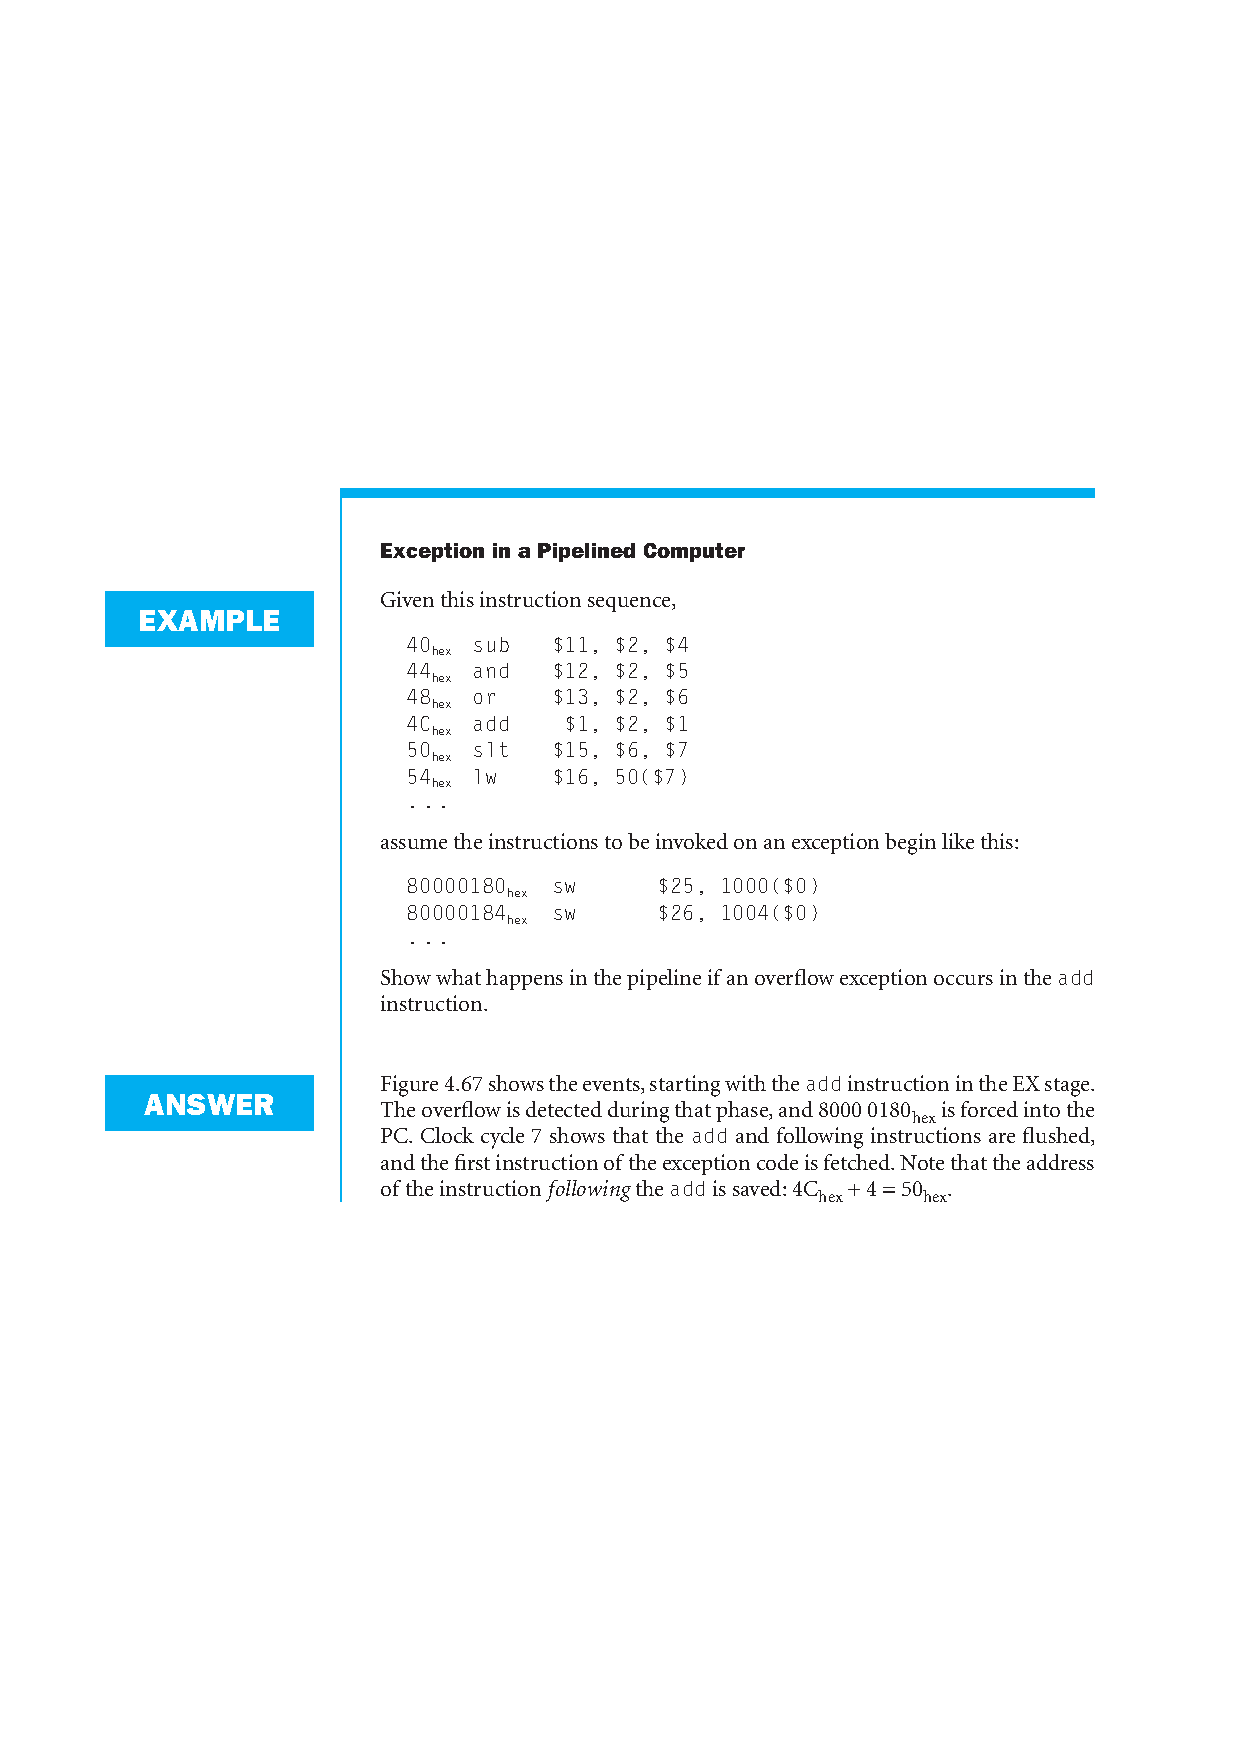
\includegraphics[scale = 0.3]{images/Example_for_Pipeline_NonExact.pdf}
					\caption{非精确处理的一个例子}
				\end{minipage}
				\\[10pt]
				\begin{minipage}{20em}
					\centering
					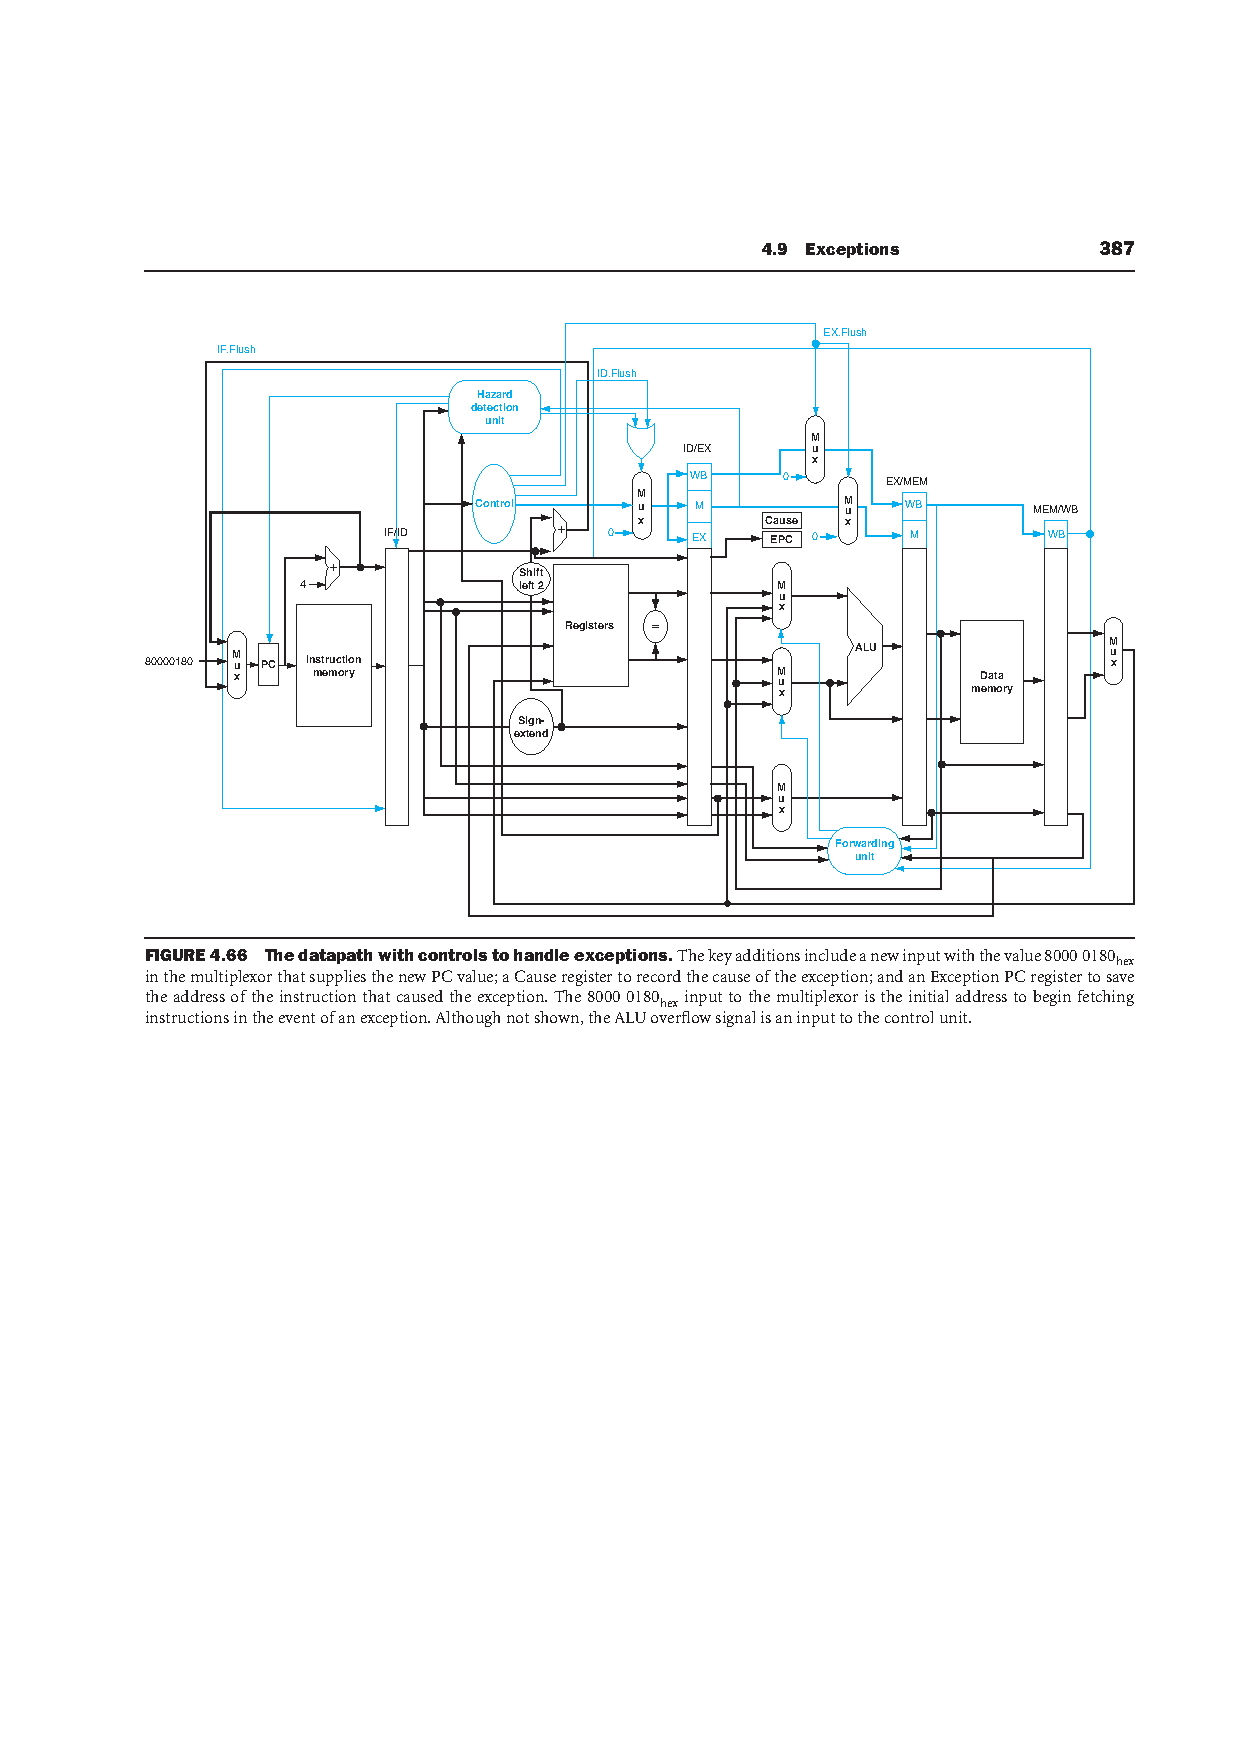
\includegraphics[scale = 0.3]{images/Pipeline_Exceptions_NonExact.pdf}
					\caption{流水线非精确处理异常的数据通路}
				\end{minipage}
			\end{minipage}
			\quad
			\begin{minipage}{20em}
				\centering
				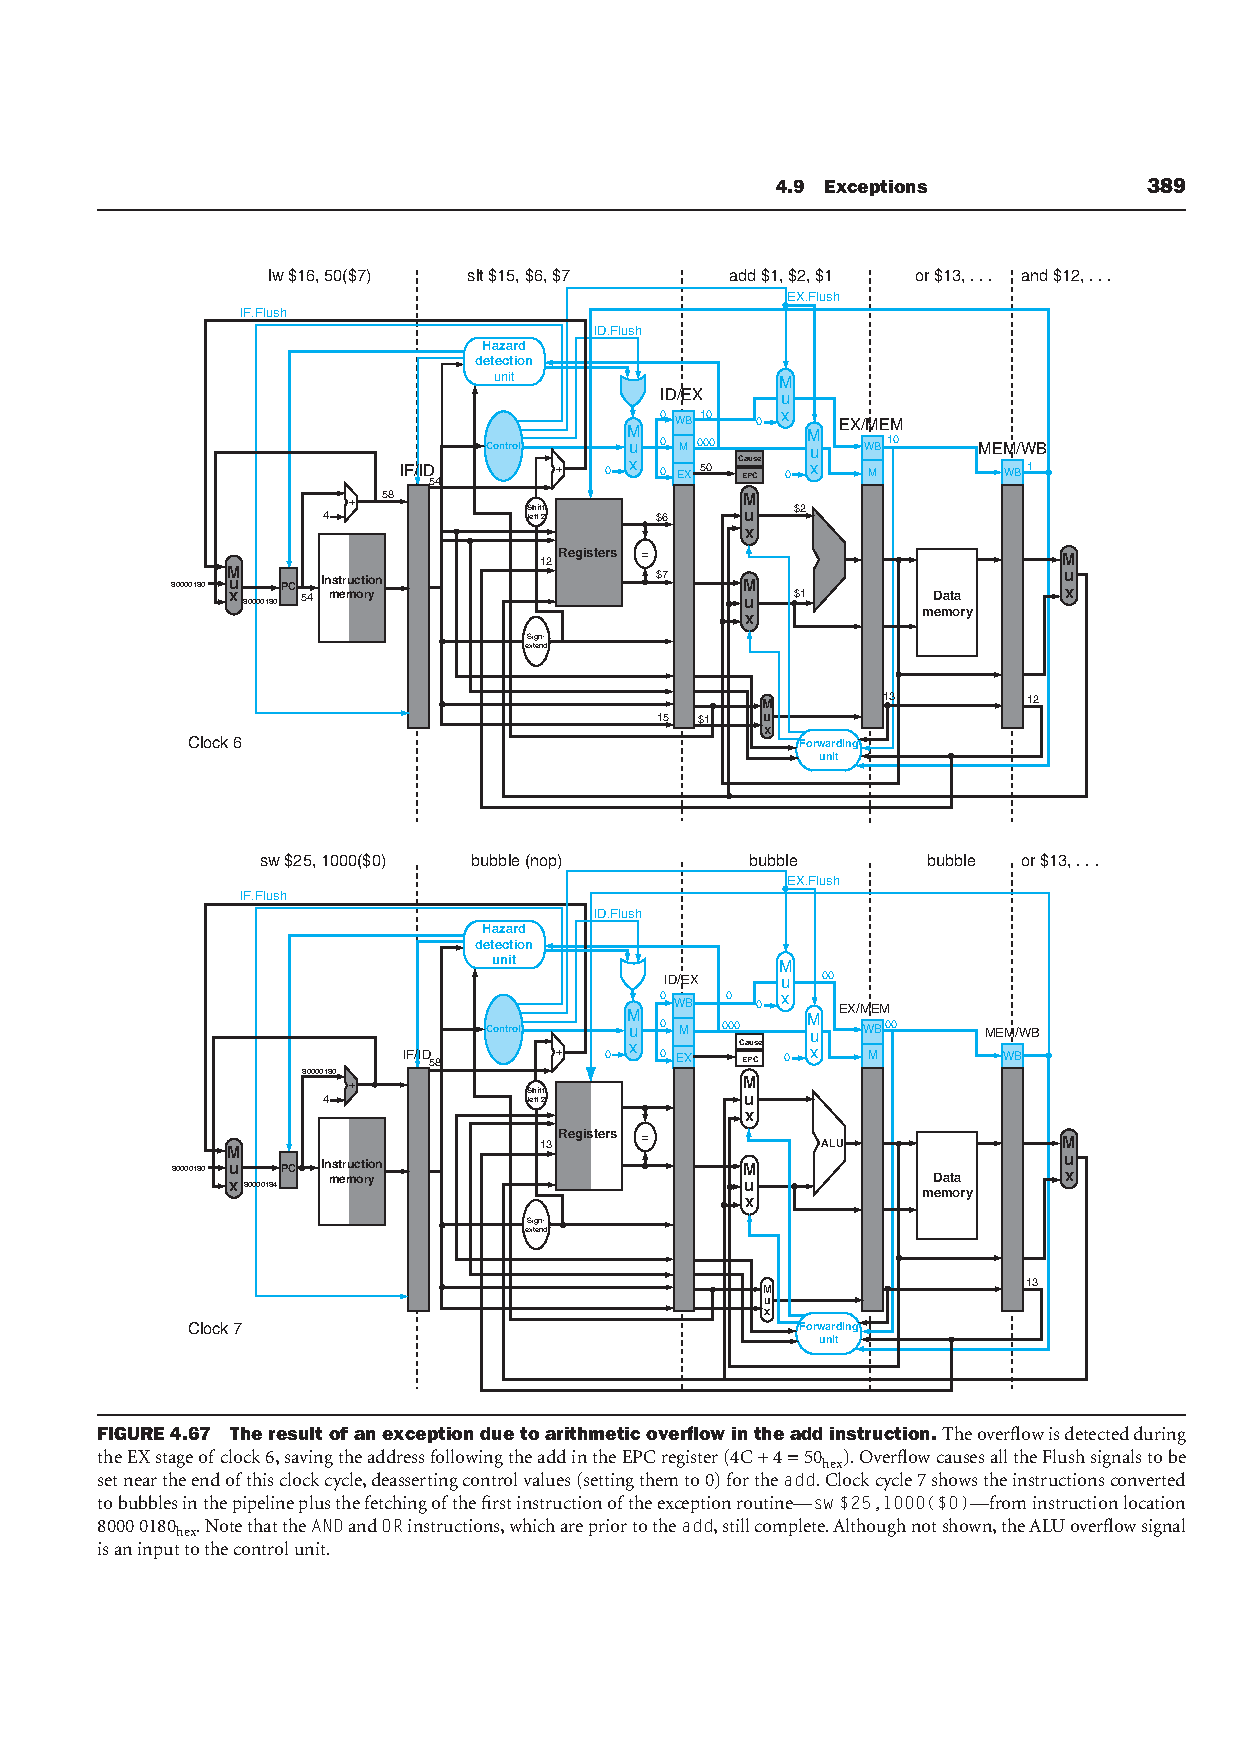
\includegraphics[scale = 0.35]{images/Datapath_of_Example_for_Pipeline_Exceptions_NonExact.pdf}
				\caption{非精确处理例题的数据通路分析}
			\end{minipage}
		\end{figure}
		\subparagraph{非精确异常的问题} Drawbacks
		\begin{enumerate}
			\item 异常响应时间较长
			\item 如果等进入流水线的指令执行结束,可能会导致程序出错
			\begin{enumerate}
				\item i: \verb|ADD R1, R2; (R1)+(R2) -> R1|,如果此时溢出?
				\item i+1: \verb|MUL R3, R1; (R3)×(R1) -> R3|,无效执行!
				\item (此处假设有forwarding)
			\end{enumerate}
			\item 程序调试不便:程序员在第 i 条指令设置断点,但程序不能准确中断在所设置的断点处。
		\end{enumerate}
		\paragraph{精确处理异常}
		遇到的困难主要是开销会很大,因为需要保证异常指令可以重启,就得做很完全的保护现场:\circled{1}\ 安全停止流水线,并完整保存当前状态\ \circled{2}\ 需要大量后援寄存器保存流水线中各指令的现场,包括RegFile、PSW、流水段寄存器(含各段的控制寄存器)。MIPS采用\textbf{提交点}技术来实现:先发生的异常并不立即处理,只是被标记。每一条指令在执行过程中记录下来自己在哪一个阶段出了错,这些错在WB段结束之后再去处理。这样做就像前面要求 \verb|R-type| 指令也要到第五个周期写回是类似的思想,统一的处理位置使得先进入流水线的指令可以先处理问题。EXCn寄存器:保存异常类型。流水线中最深的指令引起的异常最优先。直到\textsf{MEM}段才Flush
		\begin{enumerate}
			\item 保持流水线的异常标记直到提交点(MEM段)
			\item 如果提交点有异常,则更新cause和EPC,清除所有流水段,新PC值到fetch段
			\item 早期流水段的异常抑制后来的异常(flush IF/ID/EX)
			\item 提交点处引入中断处理
		\end{enumerate}
		\begin{figure}[h]
			\centering
			\begin{minipage}{40em}
				\centering
				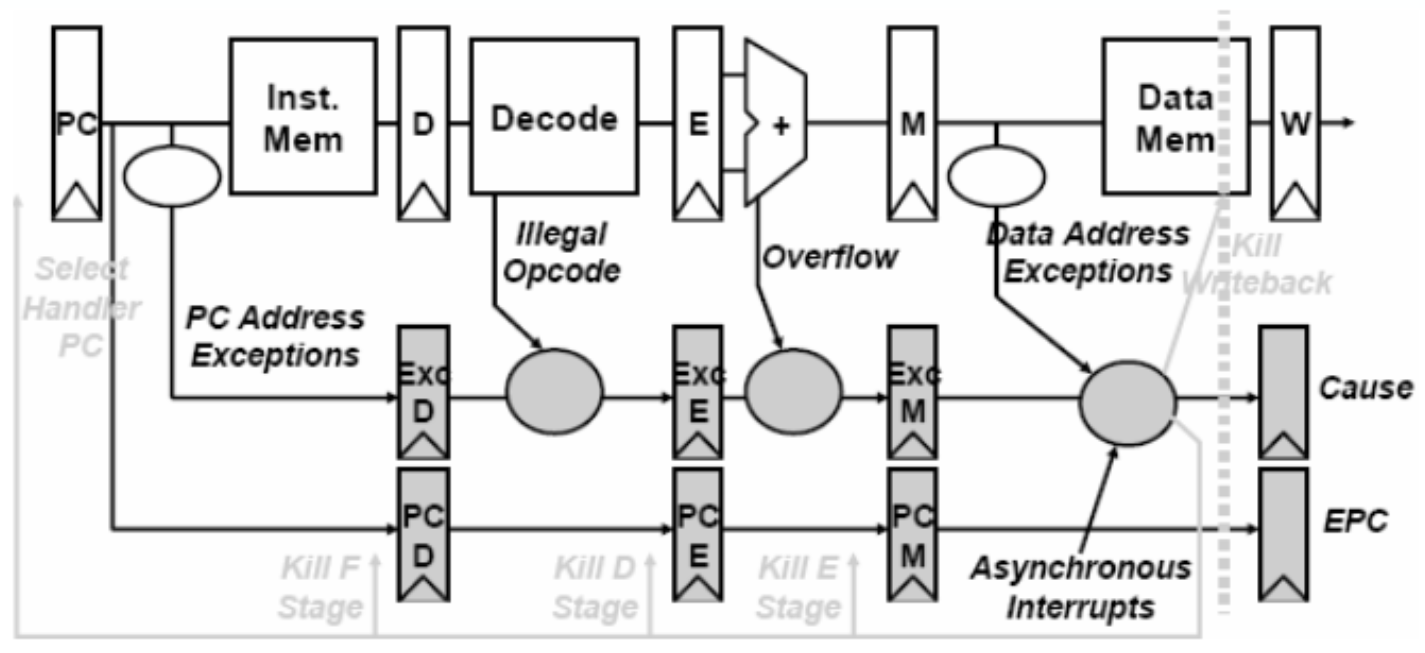
\includegraphics[scale = 0.23]{images/Pipeline_Exception_Exact.png}
				\caption{提交点和两条流水线}
			\end{minipage}
		\end{figure}
		\subparagraph{两条流水线} 提交点方案可以被看作是两条流水线,其中一个是之前普通的流水,另一个则是用于收集并在MEM段处理在各段发生的异常。这是因为不能保证前面的段出错了后面不再出错,所以每一级都需要有接收;另一个原因是在同一时钟周期,每一级流水段中是不同的指令。为了简单起见,每一条指令只保留最先发生的异常,即上文的第三条策略。
		\subparagraph{为什么要在MEM段提交} 前提:WB段不会出错
		\begin{enumerate}
			\item (需要异步在统一的段处理)都在MEM段才处理,则可以使处理顺序即为流水指令顺序,保证一个FCFS的顺序,即先进入流水线的指令先进入异常处理程序
			\item (EX段不可以)在MEM段还有可能出错,且放到MEM段可以保证前一条指令已执行完成
			\item (WB段不可以)后续指令被flush (kill),保证没有指令完成写回
		\end{enumerate}
	\subsection{容错与校验}
		基本解决方案是冗余Redundancy,用时间和/或空间的代价来换取信息的正确性,主要包括Information redundancy信息冗余(海明码、CRC码、奇偶校验码)、Time redundancy时间冗余(回滚)、Physical redundancy空间冗余(复用、磁盘冗余阵列)
		\paragraph{码距纠错理论} 理论分析纠错方法的可行性。比如校验一组数据的传输是否正确,L就是传送的数据和收到的数据之间的码距d的最小值(因为每一位都有可能翻转,所以说一般来说是只有一位错误的时候,再加上校验位的翻转数量是L)
		\begin{enumerate}
			\item 一个编码系统中任意两个合法编码(码字)之间不同的二进数位(bit)数叫这两个码字的码距,也称为汉明距离,用d表示。例如码字10010和01110,有3个位置的码元不同,所以d = 3。
			\item 整个编码系统中任意两个码字的的最小距离就是该编码系统的码距。任何一种编码是否具有检测能力或纠错能力,都与编码的最小距离有关。
			\item 在一个码组内为了检测D个误码,需要最小码距 $L\ge D+1$
			\item 在一个码组内为了纠正C个误码,需要最小码距 $L\ge 2C+1$
			\item $L-1 \ge D+C$ 且 $D\ge C$
			\item 即编码最小距离L越大,则其检测错误的位数D也越大,纠正错误位数C也越大,且纠错能力恒小于或等于检测能力。
			\begin{enumerate}
				\item 例如,L = 2,则D = 1,C = 0。码距 = 2才能检测1位错
				\item 例如,L = 3,则D = 2,C = 0;或D = 1,C = 1。码距 = 3才能检测2位错,或者检测1位错,纠错1位。
			\end{enumerate}
		\end{enumerate}
		\paragraph{奇偶编码校验} 在被传送的n位代码 $b_{n-1}b_{n-2}\cdots b_1b_0$ 上增加一位校验位P (Parity)。奇校验是使1的个数为奇数,偶校验反之。可以检测一位错
		\paragraph{Hamming码} 海明码是可以一位检验一位纠错的
			\subparagraph{写出海明码 $H_n\cdots H_1$}
			假如说有k位数据 $D_k\cdots D_1$,那么海明码的位数r需要满足 $2^r-1\ge k+r$。另一种考虑的perspective是,从最右端 ($H_1$) 开始写,下标为 $2^i$ 则填 $P_{i+1}$,其余位置顺序填 $D_j$。当数据都填完的时候就得到一个Hamming码数组(下表前两行
			\subparagraph{计算校验位} \textbf{下面都假设是偶校验,如果是奇校验那么得到的校验位再取一次反}
			首先填入每一位的校验位号。规则为该下标的二进制表示中1的位置,即为此海明位所用到的校验位。如$H_7$,$7_{Dec}=(111)_{Bin}$,则它用到的校验位为$P_1,P_2,P_3$,即$H_1,H_2,H_4$。这时候从另一个角度来看,就是每一个校验位在除了自己以外的一些位$i_1,\cdots,i_k$被用到,那么校验位的值就是$\sum H_{i_k}$,求和为$F_2$域上求和,即异或$\oplus$。如$P_1=D_4\oplus D_2\oplus D_1$
			\begin{table}[h]
				\centering
				\begin{tabular}{c|*{7}{c}}
					\toprule
					Hamming码位号& $H_7$ & $H_6$ & $H_5$ & $H_4$ & $H_3$ & $H_2$ & $H_1$ \\
					\midrule
					数据位/校验位& $D_4$ & $D_3$ & $D_2$ & $P_3$ & $D_1$ & $P_2$ & $P_1$ \\
					数值(先填入数据位)&&&&&&&\\
					参与检验的校验位号& 1,2,4 & 2,4 & 1,4& 4 & 1,2 & 2 & 1 \\
					\bottomrule
				\end{tabular}
			\end{table}
			\subparagraph{接收端校验}
			检验数位数等于校验位位数。检验数计算规则为$S_i=P_i\oplus\sum H_{i_k}$,即校验位异或所有用到这个校验位的数据位(都是接收到的值)。如$S_1=P_1\oplus D_4\oplus D_2\oplus D_1$。然后检验数$S_r\cdots S_1$的十进制值$x$就表示$H_x$是错误的
		\paragraph{CRC循环冗余码}
			\subparagraph{模2运算} 没有借位和进位。记住 $0-1=1$ 然后乘除法都老实列竖式算就OK。比如说除法,上0还是1就是看第一位
			\subparagraph{CRC的生成} 校验位与海明码不同,统一放在数据位的后面。\newline
			已知:n位原始数据和k + 1位生成多项式。
			\begin{enumerate}
				\item 在数据后面添加$k$个0,变成$n+k$位
				\item 将得到的这个二进制数除以生成多项式,得到商和余数(模2运算)
				\item 把余数补在n位数据后面,得到$(n+k,n)$码
			\end{enumerate}
			\subparagraph{CRC的错误与余数循环} 用接收到的n + k位数据串模2除生成多项式,得到一个余数。如果某一位出错,则余数不为0。不同位出错,余数不同,余数和出错位之间的对应关系不变。与待测码无关,与生成多项式有关。这个余数具有一个循环特性,即对余数补0,再除以生成多项式,便得到错误位左移一位的那个余数
			\subparagraph{纠错办法} 一个是把整张错误-余数对照表列出来,然后对比余数得到错误位。另一个是用所谓的循环移位法。
			\begin{enumerate}
				\item 将CRC码进行左循环移位,至出错位被移至最高位,即
				\begin{enumerate}
					\item 将接收数据模2除以生成多项式,得到一个余数
					\item 将这个余数右边补0,除以生成多项式,得到一个新的余数,同时把接收数据左移一位,即 \verb|CRC_next <= {CRC_curr[WIDTH-2:0], CRC_curr[WIDTH-1]}|,亦即将数据看成一个循环队列
					\item 直到得到的余数等于最高位出错时的余数(这个可以单独算一下,把原始数据最高位取反然后除以生成多项式)
				\end{enumerate}
				\item 对最高位取反纠错
				\item 继续左循环移位,直到余数和一开始的相等
			\end{enumerate}
			原理:余数和CRC码在开始移位之后便相互独立,余数的补0除实际上是一个计数器的作用,判断错误位转到最高位以及循环一周。有一点像转魔方,转到某一个样子之后做一个处理,然后恢复不需要改变的块的位置
	\subsection{Cache}
		cache是全硬件实现,注意和虚存的软件实现相区分。cache只有很少的OS参与量
		\paragraph{思考这4个各自的优点} 根据不用的应用特征,执行的轨迹或者数据通路、需要的数据量及其相关程度,以及应用的场景来选择不同的有针对性的cache
		\begin{enumerate}
			\item 单一Cache和多级Cache
			\begin{enumerate}
				\item 单一Cache:CPU和主存之间只设一个Cache。随着技术发展,与CPU制作在同一芯片中——片内Cache。\textbf{存取速度快,不占用片外系统总线,但容量受限}
				\item 多级Cache:在片内Cache基础上,再增加一(多)级片外Cache。与CPU之间使用独立数据通路
			\end{enumerate}
			\item 统一Cache和分离Cache
			\begin{enumerate}
				\item 统一Cache,指令和数据存放在同一Cache内
				\item 分离Cache,指令和数据分别存放——指令Cache 和数据Cache
			\end{enumerate}
		\end{enumerate}
		\paragraph{Cache与Memory的地址映射} 地址映射是将主存地址定位到Cache地址的方法,Cache大小要小于主存大小,且数据传输的最小单元是块,但是CPU取数据是以字为单位的。联想一下OS里面page的概念(虽然那个是内存对于硬盘而言的)。CPU给出来的是在内存里面的字/字节编号,由于分块,故低位拿出来判断在一块之内的偏移量,高位拿出来判断块号。直接映射由于是把(Cache块数)个块绑成一组平行映射到Cache,那就类似的再次高低位拆分检索,标记位数缩短
			\subparagraph{全相连映射} \textit{适用于小容量的Cache。}设主存共有$2^s$个块,每一个块里面又有$2^w$个字(或字节),那么cache就要有每一个block都能够偏移寻址到整个内存的能力,所以维持一个标记表:cache里面每一块的标记处存着这一块对应在内存里面的块号(块里面就对应把整个块的内容都copy下来)。为了快速检索,内存地址的块号与 Cache中所有行的标记同时进行比较。\textit{优点:冲突概率小,Cache的利用高。 缺点:比较器难实现,需要一个访问速度很快代价高的相联存储器}
			\subparagraph{直接映射} \textit{适合大容量的Cache。}每个主存块只能映射到Cache的一个特定块位置,每个Cache块可以和若干个主存块对应。$i$表示Cache块号,$j$表示主存块号,$m$表示Cache的总块数(一般为2的幂数),则$i = j \mod{m}$。判断命中的时候,先由块号的低位\textit{优点:比较电路少,硬件实现简单,Cache地址为主存地址的低几位,不需变换。缺点:冲突概率高}
			\subparagraph{组相连映射} \textit{是前两种方案的折中考虑。}将Cache块分为u组,每组有v块,主存块存放在哪个组是固定的,而存到组内哪个块则是灵活的:间直接映射,组内全相联映射。Cache块数 $m = u\times v$;组号 $q = j \mod{u}$:主存的第j块内容映射到Cache的第q组中的某块(v = 1,直接映射;u = 1,全相联映射)\textit{v的取值一般是2的幂,称之为v路组相联cache}
			\subparagraph{联想OS} 想一下进程调度里面,允许踢出其他进程的page就像全相连映射,可以将内存中的一个block映射到随便哪一个位置。只可以踢出自己frames里面的页,如果有好多页就像是组相连映射,同组之内可以有轮转的算法
\end{document}
